\chapter{Introduction}
\label{chap:1_introduction}
This chapter presents the motivation that led to the development of the proposed work, as well as a review of the state of the art, to achieve a general panorama of the problems and methods that this work addresses. Later, the general objectives of the developed system are outlined, with a summary of the structure of the work.


\section{Motivation}
	
Last decades, the production prices of digital cameras and high-resolution sensors have been greatly reduced, bringing these devices into the consumer market segment: nowadays, everybody carries at least 2 cameras in their mobile phone, aside of high-quality web cameras, or even driving-assistance cameras in cars. This, beside an increase in the hardware performance has resulted in a strong drive for the computer vision research (\autoref{fig:1_cv_forecast}): there are many possibilities out of industrial environments for applications using cameras, such as fancy image modifications, or autonomous driving, as it can be seen on \autoref{fig:1_computer_vision_applications}.

\begin{figure}[h]
	\centering
	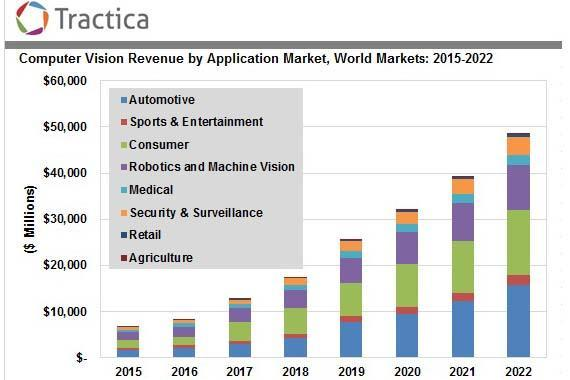
\includegraphics[width=0.8\linewidth]{cv_forecast_2022}
	\caption{Computer Vision revenues in the last year, and forecast for 2022 (source: \cite{cv_forecast}).}
	\label{fig:1_cv_forecast}
\end{figure}


\begin{figure}[h]
	\centering
	\begin{subfigure}[t]{0.45\linewidth}
		\centering
		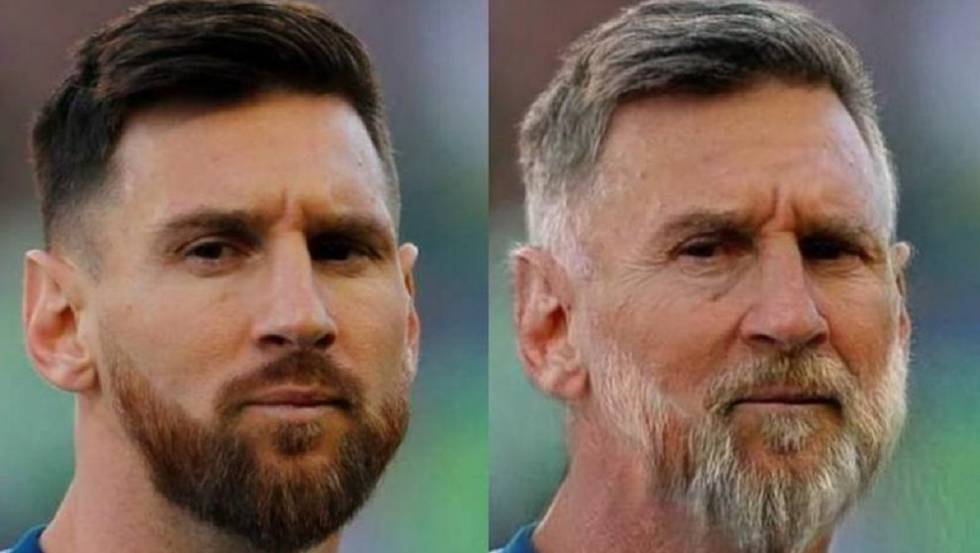
\includegraphics[width=0.8\linewidth]{faceapp_messi}
		\caption{Modifications of a subject on a portrait, such as apparent gender, or age.}
	\end{subfigure}
	\begin{subfigure}[t]{0.45\linewidth}
		\centering
		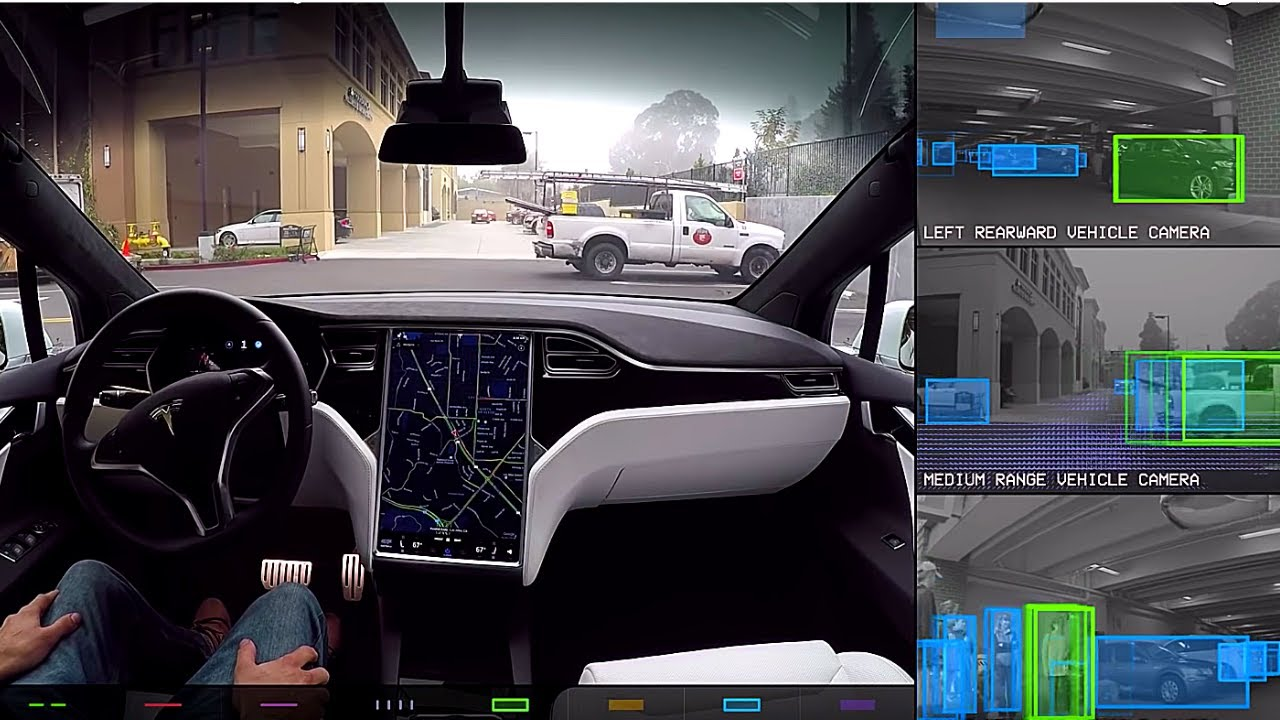
\includegraphics[width=0.95\linewidth]{tesla_autonomous_driving}
		\caption{Autonomous driving on a Tesla Model X.}
	\end{subfigure}
	\caption{Examples of contemporary computer-vision applications.}
	\label{fig:1_computer_vision_applications}
\end{figure}

Specially, the latest times have been notoriously active in this field because of the massive use of \textit{deep learning} for addressing high complexity tasks, such as language understanding \cite{gpt2}, speech recognition \cite{speech_neural} and computer vision problems, which are linked to the growing interest shown in \autoref{fig:1_cv_forecast}. This massive use began in the ImageNet classification contest, where a deep neural network system, AlexNet \cite{alexnet}, achieved an overwhelming victory over another approaches. This discovery, along with the strong advances in computing power and parallel computing have impulsed the usage of these systems, which show an outstanding performance with the available means nowadays \cite{diapos_deep_learning}.\\


On the other hand, robotics applications can be really useful at daily tasks. These tasks are of greater interest when the behavior of a robot tends to emulate the human one\footnote{\href{https://www.engadget.com/2018/01/08/new-sony-aibo-first-impressions/}{Some efforts are taken even into adopting the performance of human's best friend}}, with the advantage of no people exposed to a significant risk, or, in a less gloomy scenario, without human body physical limitations. This requires a polished (and somehow complex) behavior, which is triggered by a certain input. At this point, two main branches can be found into robotics:
\begin{description}
	\item [Teleoperated robots:] this kind of robots are capable of perform certain actions, which are \textit{remotely controlled by a human operator}. This type is the mostly used one on the hazardousness (\autoref{fig:1_pioneer}) \cite{chernobyl-robot} or precision \cite{teleop-surgery}. Some advances are made nowadays improving the teleoperation function, implementing \textit{feedback} from the robot, such as haptic feedback \cite{teleop-haptic}, or VR (\emph{Virtual Reality}) sensation, to allow that person to sense the environment as if they were in the robot position.
	
	\item [Autonomous robots:] these robots are much more complex machines, as they are distinguished for implementing a response by itself, independently of any kind of remote operator. This is seeked on certain scenarios, where there are some factors (as the time elapsed performing an action, or the cost of a control link with the robot) with a considerable weight in the design \cite{ai-space}. This is the kind of robots that concern us on this work: the state-of-the-art techniques try to emulate \textit{human behavior} (\autoref{fig:1_pepper}), so some actions can begin to be performed autonomously with a certain intelligence, as it will be describe below.
\end{description}


\begin{figure}[h]
	\centering
	\begin{subfigure}[t]{0.45\textwidth}
		\centering
		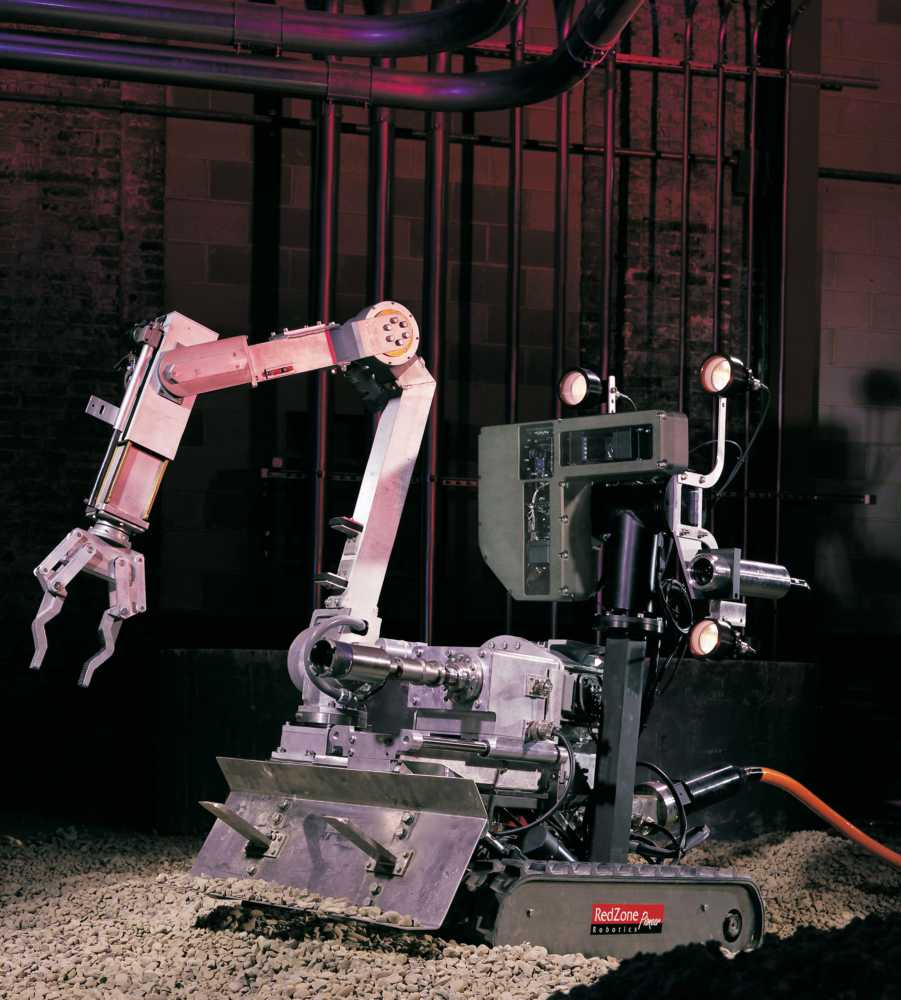
\includegraphics[width=0.8\linewidth]{pioneer_chernobyl}
		\caption{Pioneer robot, designed to perform hazardous teleoperated explorations in a deadly radioactive environment.}
		\label{fig:1_pioneer}
	\end{subfigure}
	\hfill
	\begin{subfigure}[t]{0.4\textwidth}
		\centering
		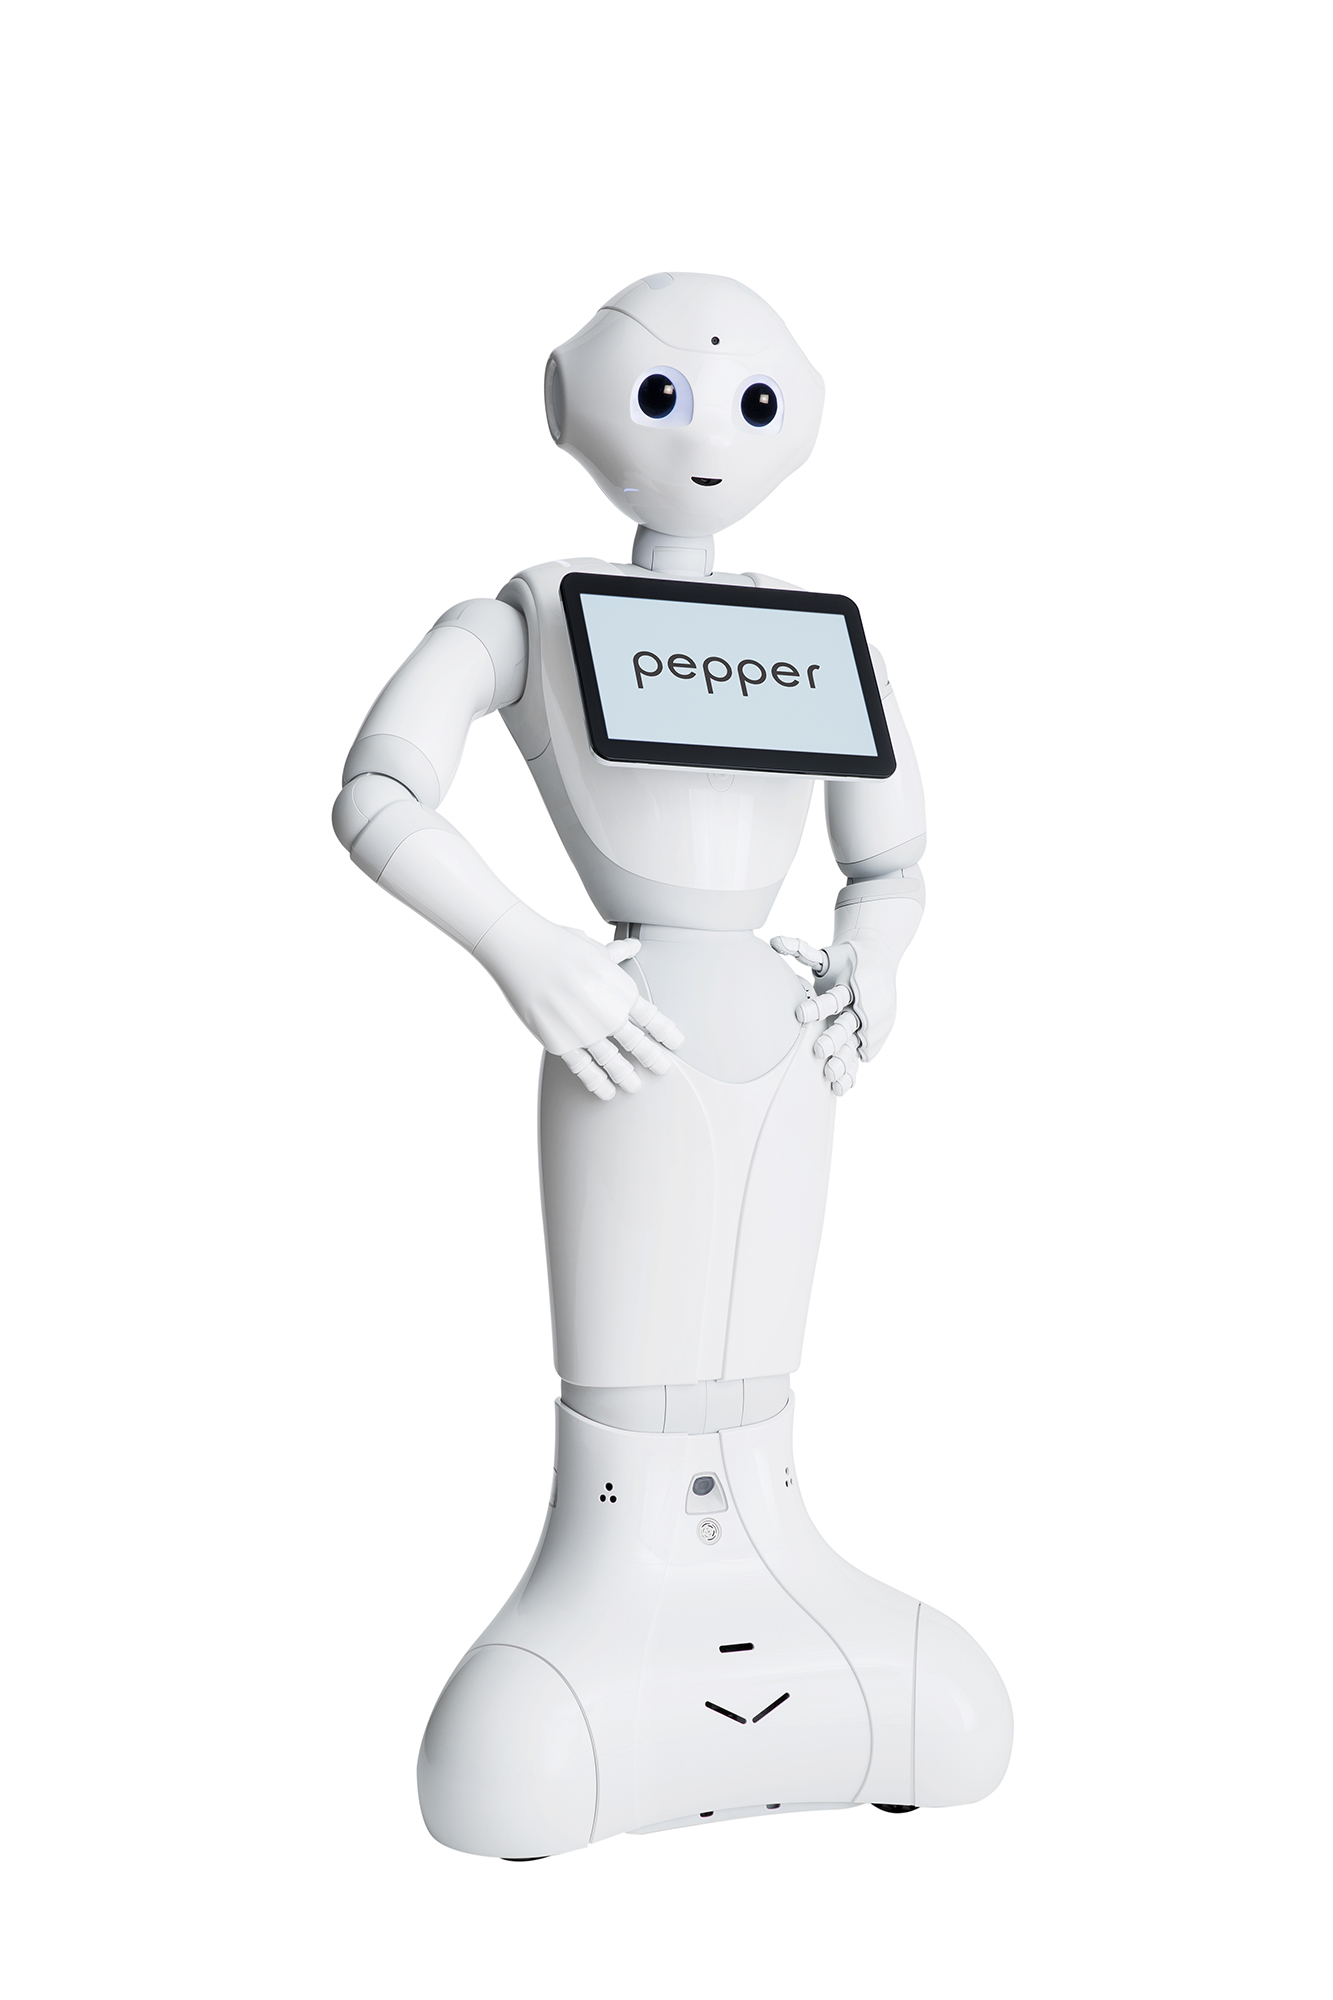
\includegraphics[width=0.8\linewidth]{pepper}
		\caption{Pepper, an autonomous humanoid capable of performing on-board processing and reacting to external stimuli intelligently.}
		\label{fig:1_pepper}
	\end{subfigure}
	\caption{Example of a teleoperated and an autonomous robot.}
	\label{fig:1_robots}
\end{figure}

The important advances on the last decades on the image processing and audio recognition fields have fostered the development of assistance systems, apart from critical machines as the previously described examples.\\



There are outstanding synergies between robotics and computer vision, as it is explored on the system proposed in this work: these fields are combined for obtaining a robust robot capable of following a certain person, navigating towards it on a reactive behavior, and using deep-learning based visual perception. This behavior is composed of two main components: the \textit{perception block}, in charge of processing the images from an RGBD camera placed on the system, and the \textit{actuation block}, which moves the robotic base accordingly to the relative position of the person to be followed.\\

This application can be specially interesting on social robots, which are designed to follow a person at home or in a hospital. According to \cite{natural_personfollowing}: \textit{robots that operate around people in the real world need to move in coherent, easily-understood ways, so that they will not startle or harm the people around them. In particular, for robots that operate in hospitals or in nursing homes}. 



The work proposed in this thesis improves the system developed on \cite{tfg}, where a neural following system was run in a standard laptop, with a camera and a robot plugged. In the following dissertation, this work will be revisited, and the points of interest which have allowed to enhance the previous version will be described.\\
	
The main contributions of this solution may be brought in as follows:
\begin{description}
	\item[Embedded solution:] the final system is mounted on a battery-powered \textit{mobile base}. This robot features a high-performance GPU embedded on a SoM (\textit{System-on-Module}). In contrast to the previous work, this assembly can operate on its own, without requiring an external computer to perform the deep learning inferences or running algorithms in parallel. A remote monitoring of the behavior is available as well, but it is not required for the system to work. In addition, specific optimization engines allow the system to run faster with 3 neural networks than previously with only 2 networks, on a low-consumption hardware. This will be reviewed in \autoref{chap:3_results}.

	\item[Person identification:] the proposed system runs 3 neural networks. These networks perform inferences over the images perceived by the RGB-D sensor, which is attached to the system as the sensing source of the robot. The inferences are devoted to detect the different persons in the scene, as well as to distinguish them by means of a discriminant feature: their face. Unlike the previous development, all the detection and identification tasks are based on neural networks, achieving greater robustness and reliability as it will be depicted in \autoref{chap:3_results}.

	\item[Tracking:] the full system includes also a person tracker based on optical flow. This aims to guess the trajectories followed by each person that the robot can see. As opposed to the previous work, this tracker allows to roughly follow the persons while the neural network yields a new update, as this tracker takes considerably less time to infer the person displacement. As a result, the robustness of the entire system is improved, compared to a version governed exclusively by the neural inferences, which are sensitive to visual occlusions as well. Trusting just on these inferences could easily result on an unsteady behavior. However, the introduction of the tracker softens the robot movements ensuring a more robust following, as it will be explained on \autoref{sec:2_functional_architecture}.
\end{description}


	
\section{State of the art}
\label{sec:1_sota}
	As it was previously introduced, this work is performed to explore the synergies on robotics and deep-learning-based visual perception. In this section, the current approaches and tools will be depicted in order to outline a general panorama where this work may be placed.\\
	
	The problem to be addressed is to \textit{get a robot with a camera to follow a person}. This problem can be split into several steps, where different approaches have been previously proposed. These steps will be covered in the following subsections.
	
\subsection{Visual person detection}


One of the most used approaches is commonly called the \textit{Viola-Jones} detector \cite{violajones}. This algorithm relies on a \textit{rigid body model}, which fits a specific shape. On a grayscale image, this shape can be typically distinguished by means of the pixel intensity levels. Several spatial filters called \textit{Haar features} (\autoref{fig:1_haarfeats}) are introduced: these are used across the image looking for the intensity pattern for each mask, which should resemble a part of the rigid body. As this presents a weak decision by itself, several filters (previously chosen in a training process) are combined on a \textit{boosted cascade} (\autoref{fig:1_violajones_boost}). A person is detected if the weighted combination of several filters are triggered inside a certain area, which is decided to potentially contain a person \cite{diapos_cv_clasif}.

\begin{figure}[h]
	\centering
	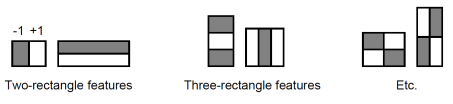
\includegraphics[width=0.7\linewidth]{haar_feats}
	\caption{Haar features: some examples \cite{diapos_cv_clasif}.}
	\label{fig:1_haarfeats}
\end{figure}

\begin{figure}[h]
	\centering
	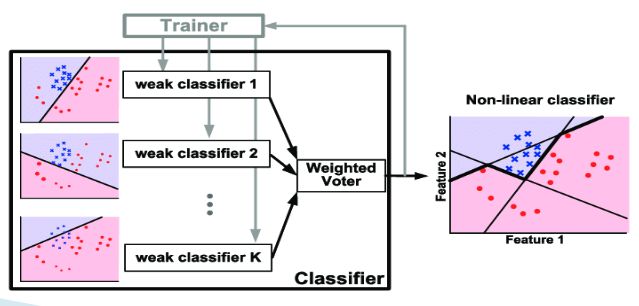
\includegraphics[width=0.7\linewidth]{boosted_cascade}
	\caption{Boosted weak classifiers \cite{diapos_cv_clasif}.}
	\label{fig:1_violajones_boost}
\end{figure}

Although this system was originally developed to detect faces, the rigid body model allows a generalization powerful enough to extend this to another object classes, \textit{person} among these. The open-source standard image processing library, OpenCV, includes pre-trained models\footnote{\url{https://github.com/opencv/opencv/blob/master/data/haarcascades}}, which can be directly used with their Viola-Jones implementation. Scale invariance can be achieved evaluating the image at multiple scales on runtime.


Another common approach nowadays for person detection is based on HoG (\textit{Histograms of Gradients}) \cite{hog_detection}. This method computes local features by means of the intensity gradients across the image, and quantizes them using their angle (creating a histogram for the oriented gradients for that pixel), as it can be seen on \autoref{fig:1_hog_sift}.\\


\begin{figure}[h]
	\centering
	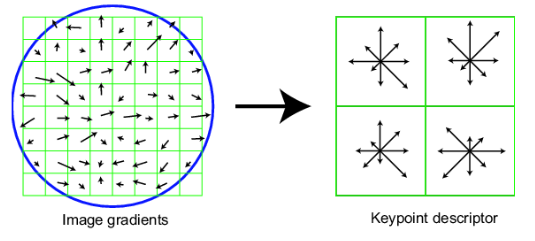
\includegraphics[width=0.7\linewidth]{hog_sift}
	\caption{Example of a HoG, quantized to 8 directions \cite{diapos_cv_features}.}
	\label{fig:1_hog_sift}
\end{figure}



These gradients are collected in $64 \times 128$ windows, and treated as features from which a linear SVM (\textit{Support Vector Machine}) is trained in order to classify a region as \textit{person/non-person}. \autoref{fig:1_hog_avg} shows the average gradient patch for a person (the direction of each gradient is not shown). A visual inspection immediately resembles the shape of a person standing up. Thus, this detector will yield the best performance when the person to be detected stands in that specific pose.

\begin{figure}[h]
	\centering
	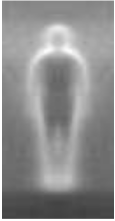
\includegraphics[width=3cm]{hog_avg}
	\caption{Average gradient for person detection on \cite{hog_detection}.}
	\label{fig:1_hog_avg}
\end{figure}



These methods, among several more, have been the state-of-the-art techniques: the cornerstone are the image gradients, which can be computed with a high efficiency,  and present decent performance. However, their main drawback is the \textit{generalization} capability, as a successful detection is highly dependent on the person pose. However, in the latest advances, the detection techniques have moved towards the spreading paradigm: \textit{deep learning}, especially the most salient tools on image processing: CNNs (\textit{convolutional neural networks}).\\

CNNs are based on standard neural networks, which combine lots of neurons or \textit{perceptrons} organizing them into layers. These perceptrons (\autoref{fig:1_perceptron}) implement non-linear operations, that allow to extract (after a proper training process) abstract features, which gain in complexity when the number of internal layers increase. When a neural network is composed by several \textit{hidden} layers (in addition to the input/output ones), it is placed into the \textit{deep learning} paradigm (\autoref{fig:1_deep_learning}).

\begin{figure}[h]
	\centering
	\begin{subfigure}[t]{0.35\linewidth}
		\centering
		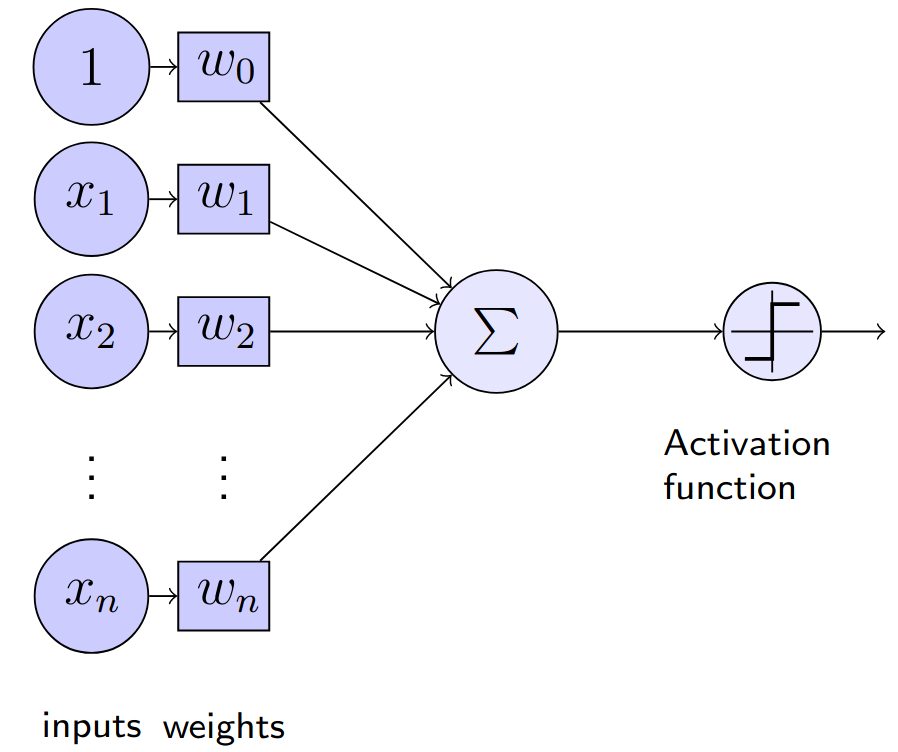
\includegraphics[width=0.95\linewidth]{perceptron}
		\caption{Basic unit of a neural network: the perceptron (source: \cite{tfg}).}
		\label{fig:1_perceptron}
	\end{subfigure}
	\begin{subfigure}[t]{0.5\linewidth}
		\centering
		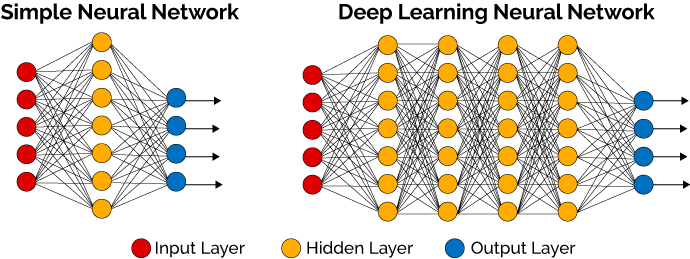
\includegraphics[width=0.99\linewidth]{deep_learning}
		\caption{Standard neural network vs. deep neural network (source: \cite{tfg}).}
		\label{fig:1_deep_learning}
	\end{subfigure}
	\caption{Basis of deep neural networks.}
	\label{fig:1_dnns}
\end{figure}

\vspace{8cm}

Based on this approach, and taking advantage of the \textit{spatial correlation} when the signal to process is an image, a neural network can be modified to implement a different operation on each perceptron: the \textit{image convolution} (\autoref{fig:1_convolution}).

\begin{figure}[h]
	\centering
	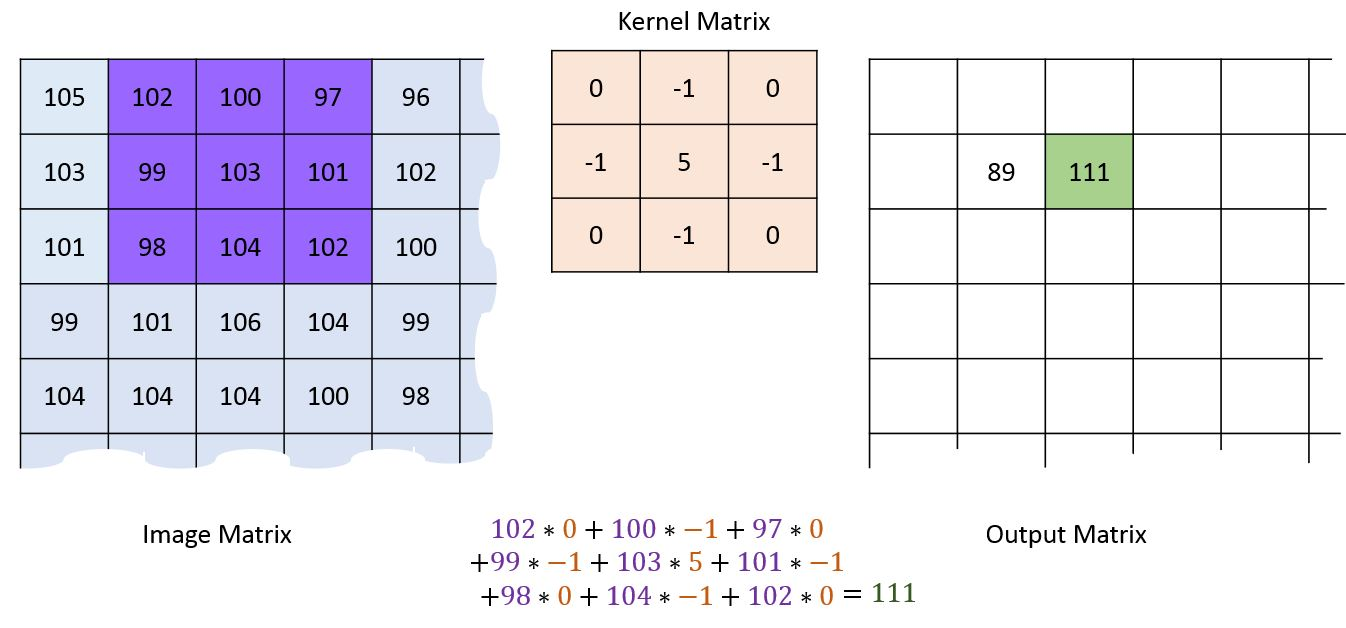
\includegraphics[width=0.7\linewidth]{convolution}
	\caption{Convolution applied on an image, applying the mask (red) on a region  (purple) of the input image, storing the result on the mapping of the central pixel of the region (green). The computation is the sum weighted by the mask values (bottom) (source: \cite{tfg}).}
	\label{fig:1_convolution}
\end{figure}

As it can be seen on \autoref{fig:1_cnn}, convolutional units may be arranged conforming a set of layers used to build \textit{feature extraction} stages (shown in red in the figure). Several layers can be concatenated, gaining in depth and obtaining more complex feature maps. These layers are finally followed by a detection/classification ensemble of \textit{dense} layers (shown in blue in the figure): a set of layers with standard perceptrons fully connected among them, yielding a final output, dependent on the classification structure of the network.

\begin{figure}[h]
	\centering
	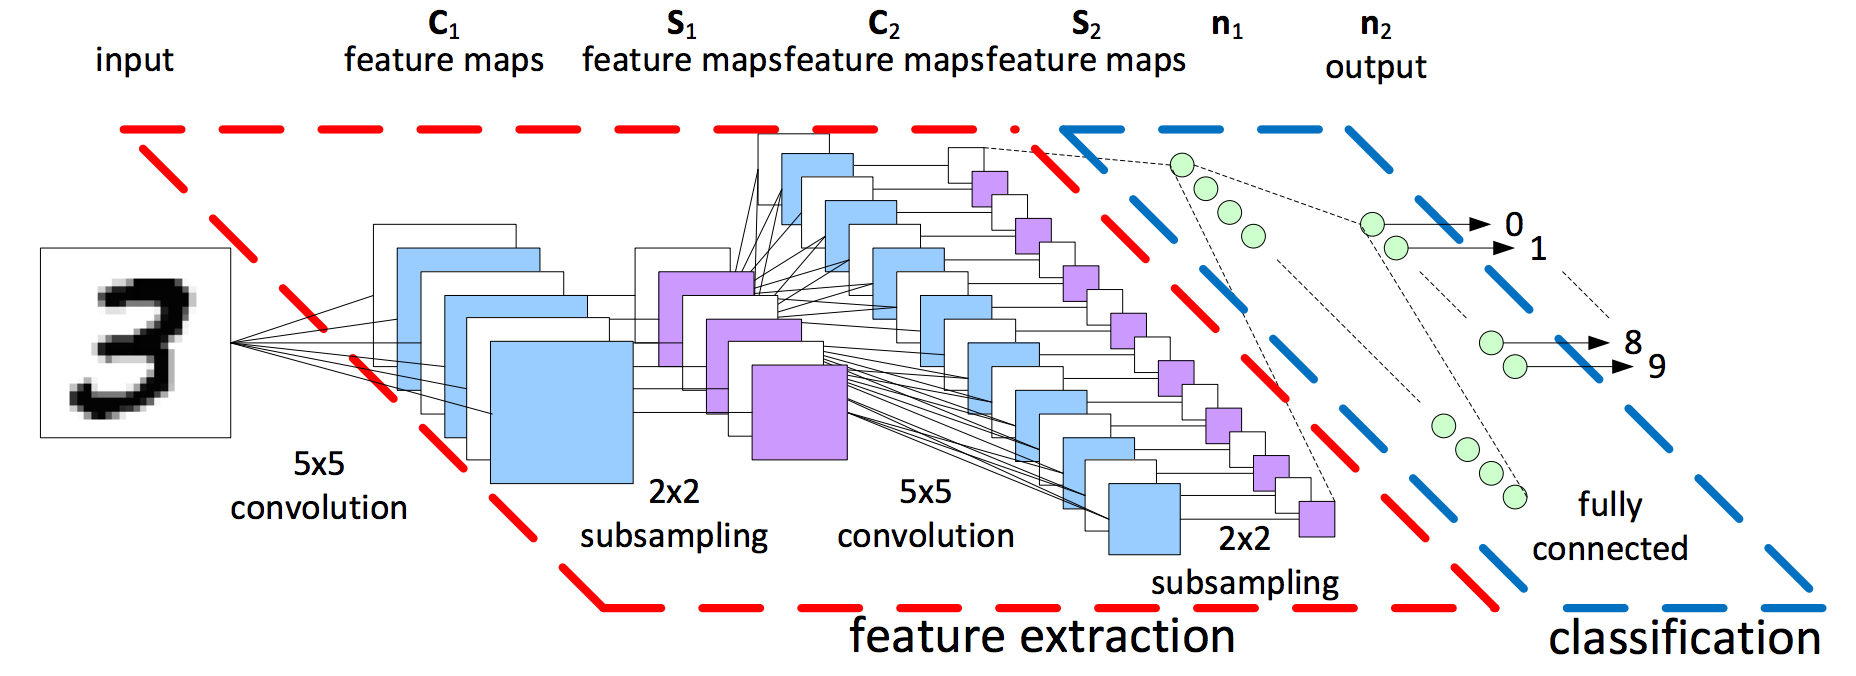
\includegraphics[width=0.9\linewidth]{cnn_architecture}
	\caption{Schematic of a digit classification CNN (source: \cite{tfg}).}
	\label{fig:1_cnn}
\end{figure}
\vspace{8cm}
In the case of object detection networks (the ones involved in this work), the output varies depending on the implementation, but it is generally composed of a set of (location, probability) tuples, one for each class the network is capable of detecting. \autoref{fig:1_activation_maps} shows the activation maps of an object detection network, where the map presents higher values in the regions with high probability of containing the object of the class it is designed for. Several of these maps compose each neuron on a CNN.

\begin{figure}[h]
	\centering
	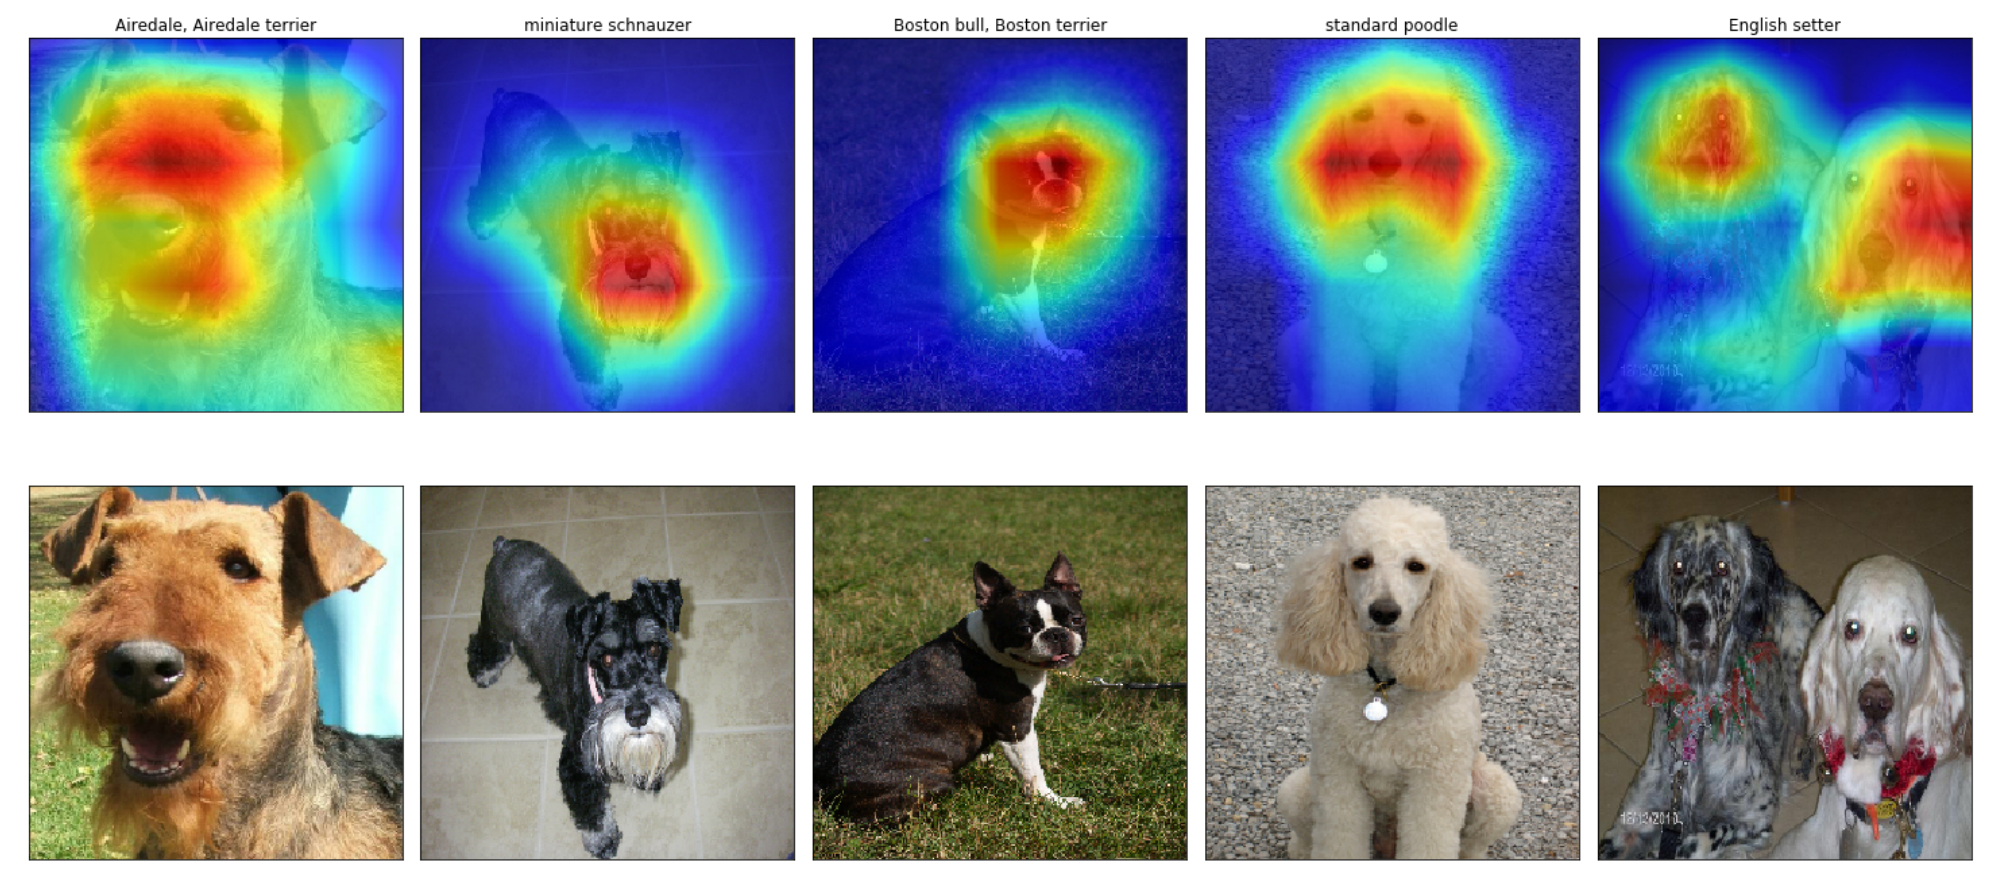
\includegraphics[width=0.9\linewidth]{activation_maps}
	\caption{Activation maps of a detection CNN searching for dogs on different images (source: \cite{tfg}).}
	\label{fig:1_activation_maps}
\end{figure}


One possible application of this concept is focused on what is called \textit{Region-based Convolutional Neural Networks} \cite{rcnn}, which require a previous step on the image called \textit{region proposal}. This step is devoted to find potential regions on the image to contain an object. This way, the challenge is to label these region according to the objects contained inside, reducing the problem to a classification task. However, the process to find these undetermined regions and iterate over them makes the process too slow for real-time requirements, which are explicitly contained in our requirements. Care has been put in posterior works \cite{fastrcnn} \cite{spp} to reduce this computation time. However, this reduction in time brings about a reduction in precision as well.\\



\subsubsection{SSD}

Another outstanding object detection architecture is SSD (\textit{Single-Shot Multibox Detector}) \cite{ssd}. The main benefit from this architecture is the fact that it embeds all the required computations in a single neural network, reducing the complexity compared to other approaches requiring external region proposals, as it was depicted above. This greatly reduces the computational time when the network has to evaluate an image. The architecture can be seen at \autoref{fig:1_arch_ssd_yolo}, and can be split into stages \cite{tfg}:

\begin{description}
	
	\item[Reshape:] the posterior stages evaluate the images on a fixed tensor size of $n \times 300 \times 300 \times 3$ (being $n$ the size of the input batch). Other image sizes might be used, however this one offers a good trade-off between score and computational load.
	
	\item [Base network:] this first group of layers are reused from a typical image classification model, such as VGG-16 \cite{vgg16}. The first layers from this architecture are utilized in this design, truncated before the first classification layer. This way, the network can leverage the \textit{feature maps} from the classification network, in order to find objects inside the input image. At the output of this network, several convolutional layers are appended, decreasing in size. This has the objective of predict detections at multiple scales. One thing to mention at this point is that the base network can be a different one rather than VGG-16, such as a MobileNet \cite{mobilenet}, which is highly optimized for running on low end devices. This is interesting as our embedded system will be limited in computing power. It will be revisited in future sections.
	
	\item[Box predictors:] for each extracted set a dedicated operation is performed, generating a small set (typically 3 or 4) of fixed-size \textit{anchors}, with varying aspect ratios for each cell on a grid over the activation map (\autoref{fig:1_ssd_generated_boxes}). As these maps have different sizes, this aims to detect  objects in different scales. The anchors are then convolved with small filters (one per depth channel), which output \emph{softmaxed} confidence values for each known class, and offsets for the generated bounding box. So, for each detected object (on that scale), the network computes the score for each class and its estimated position inside the feature map (hence, in the image as well).
	
	\item [Postprocessor:] as several detections might be triggered in the same area for different classes and scales, a \textit{Non-Maximum-Supression} \cite{nms} operation is performed at the output of the network to retain the best boxes, under a combined criteria of detection score and IoU score (\textit{Intersection over Union}), which measures the overlapping quality between two bounding boxes, as it can be seen in \autoref{fig:1_iou}.
\end{description}

\vspace{8cm}
\begin{figure}[h]
	\centering
	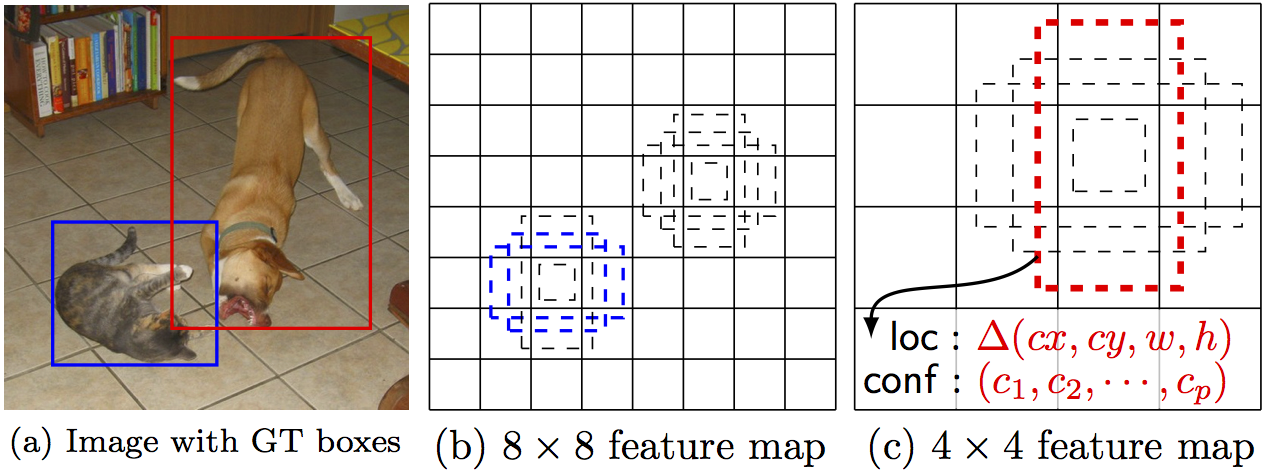
\includegraphics[width=0.7\linewidth]{ssd_generated_boxes}
	\caption{A set of boxes are generated centered on each point of every feature map \cite{ssd}.}
	\label{fig:1_ssd_generated_boxes}
\end{figure}

\begin{figure}[h]
	\centering
	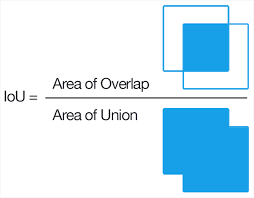
\includegraphics[width=0.4\linewidth]{iou}
	\caption{Graphical representation of the IoU score between two bounding boxes.}
	\label{fig:1_iou}
\end{figure}

\subsubsection{YOLO (You Only Look Once)}

Another interesting approach on the neural networks field is the YOLO (\textit{You Only Look Once}) system \cite{yolov1}. Its main advantage is its inference speed, due to the fact that it performs a single analysis on the entire image, dividing it into a grid of cells. Each cell predicts up to 5 boxes, containing an \textit{objectness score} (the predicted IoU of the proposal with an object, regardless its class), the coordinates of the bounding box, and a probability for the object belonging to each class. This design run faster than other methods \cite{yolov1}, however it presents a poor performance when detecting small objects.\\

This design was revisited in YOLO9000 \cite{yolov2}, introducing several improvements such as batch normalization on the input of the convolutional layers, or the concept of \textit{anchor boxes}: the box proposals follow a fixed set of aspect ratios, chosen previously using clustering on a training set. As it can be seen on \autoref{fig:1_yolov2_anchor_clustering}, limiting the proposal shapes to 5 fixed sizes improves the performance while maintaining a high IoU metric. A visual inspection shows that the selected anchors seem like a reasonable shape for the majority of the objects the network aims to detect. Additionally, the number of deep layers was increased from 26 layers to 30, and a semantic modeling is performed on the labels across different datasets, allowing the network to be trained in different datasets under a common semantic structure called \textit{WordTree} (\autoref{fig:1_yolov2_wordtree}).

\begin{figure}[h]
	\centering
	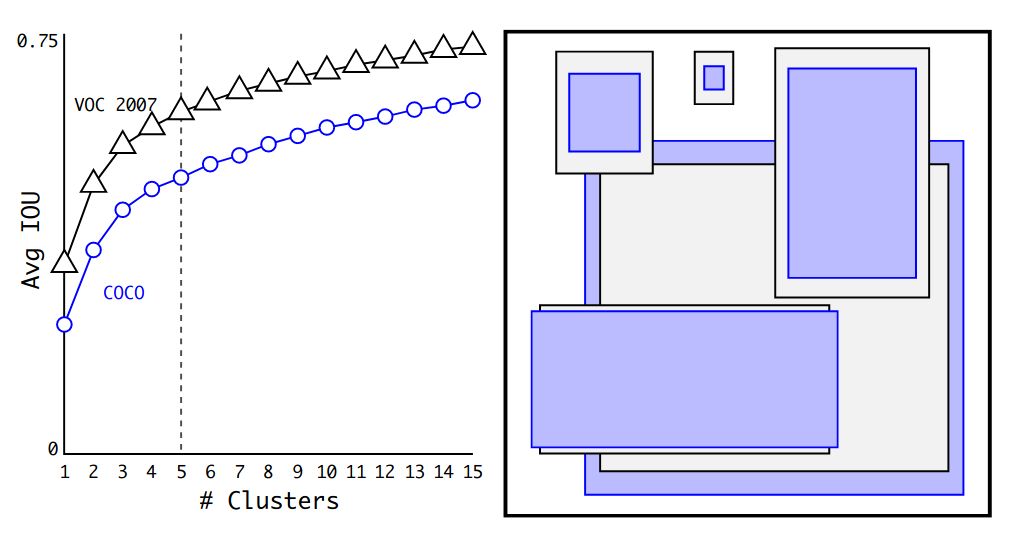
\includegraphics[width=0.6\linewidth]{yolov2_anchor_clustering}
	\caption{Result of the anchor k-means clustering on VOC and COCO for YOLO9000. Using $k=5$ anchor sizes on the right yields a good tradeoff between simplicity and improvement on the obtained IoU with respect to using $k-1$ clusters (source: \cite{yolov2}).}
	\label{fig:1_yolov2_anchor_clustering}
\end{figure}
\vspace{8cm}
\begin{figure}[h]
	\centering
	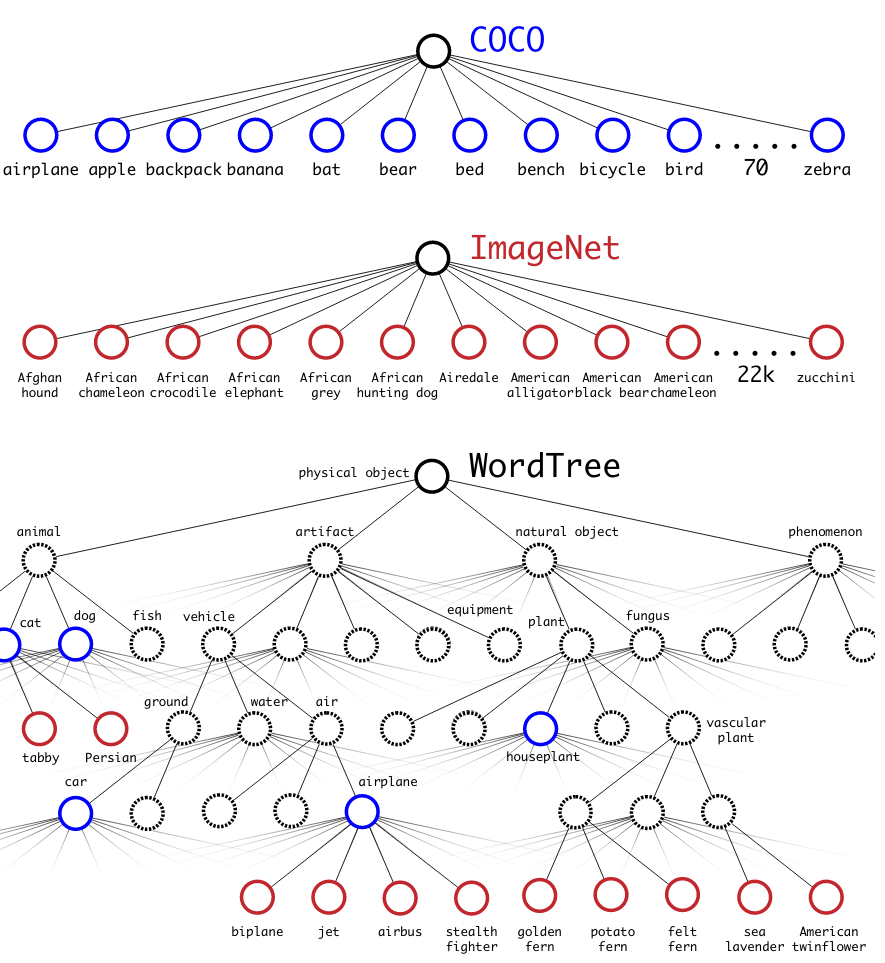
\includegraphics[width=0.6\linewidth]{yolov2_wordtree}
	\caption{Comparison between simple labeling structures (top) and a WordTree semantic grouping under categories. This allows to follow a dataset-agnostic training process as the labels can be combined using WordTree.}
	\label{fig:1_yolov2_wordtree}
\end{figure}




The latest improvement of YOLO, YOLOv3 \cite{yolov3}, features residual networks \cite{resnets}, which tackle the problem of \textit{vanishing gradients} when the networks become deeper. The stacking of several layers results on gradients diminishing its value up to a point the precision mode of the machine is not able to handle. The gradients are canceled, burdening the training process, as the first layers parameters take a substantially higher time to converge. The residual networks added in this revision of the design add shortcut connections across the layers, centering the backpropagation gradients on 1. As this reference states \cite{yolov3}, the combination of these residual layers and convolutional ones allows to train much deeper architectures (53 convolutional layers), capable of yielding a higher generalization. As in the SSD detectors, the YOLO architecture performs multi-scale detections, using 3 scales for splitting the feature maps into cell grids. A similar k-means than in \autoref{fig:1_yolov2_anchor_clustering} is performed on the COCO dataset, selecting 9 anchor sizes instead of 5, and grouping them in 3 scales. Now, on each of the cells, 9 anchor bounding boxes are fit (3 anchor shapes $\times$ 3 scales). This aims to solve the poor performance of the previous version when dealing with small objects, as well as a better generalization: in the R-CNN \cite{rcnn} and the SSD \cite{ssd} the anchor shapes are hand-picked. These changes, with a tuning on the error function, conform the YOLOv3 improvements over the previous versions.\\

For each (anchor, cell, scale) combination, this network predicts:

\begin{itemize}
	\item The coordinates of the object inside the anchor. Details can be visualized on \autoref{fig:1_yolo_output}.
	
	\item \textit{objectness} score, which is computed by means of a logistic regression in order to determine the probability of overlap with a ground truth bounding box more than any other prior anchor.
	
	\item 80 scores, as the original implementation is trained in the COCO dataset, which contains 80 classes. These classes might be overlapping (e.g. ``woman" and ``person"). Thus, these scores are computed by independent logistic classifiers and are not passed through a \textit{softmax} operation.
\end{itemize}


\begin{figure}[h]
	\centering
	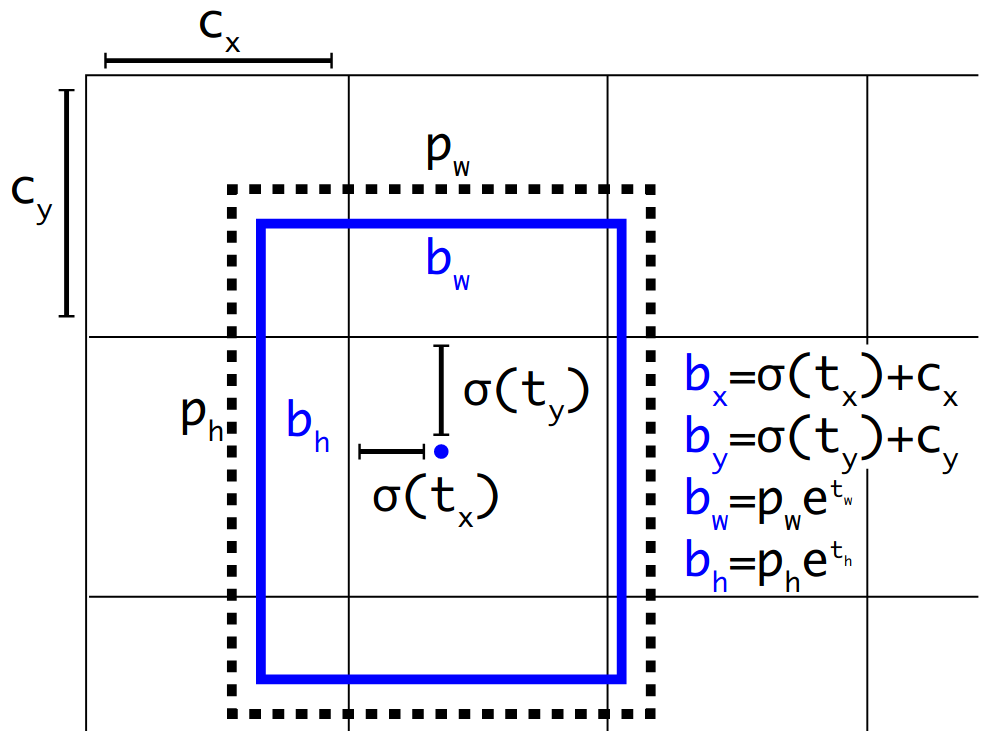
\includegraphics[width=0.5\linewidth]{yolo_outputs}
	\caption{Output on YOLO for each anchor and cell. The dashed line represents the prior anchor, while the blue line represents the detection which corrects that anchor.}
	\label{fig:1_yolo_output}
\end{figure}


The architecture of a YOLO-based detection network can be seen beside a SSD-based one in \autoref{fig:1_arch_ssd_yolo}. This allows to see the fundamental difference in the feature extraction stage of each approach.

\begin{figure}[h]
	\centering
	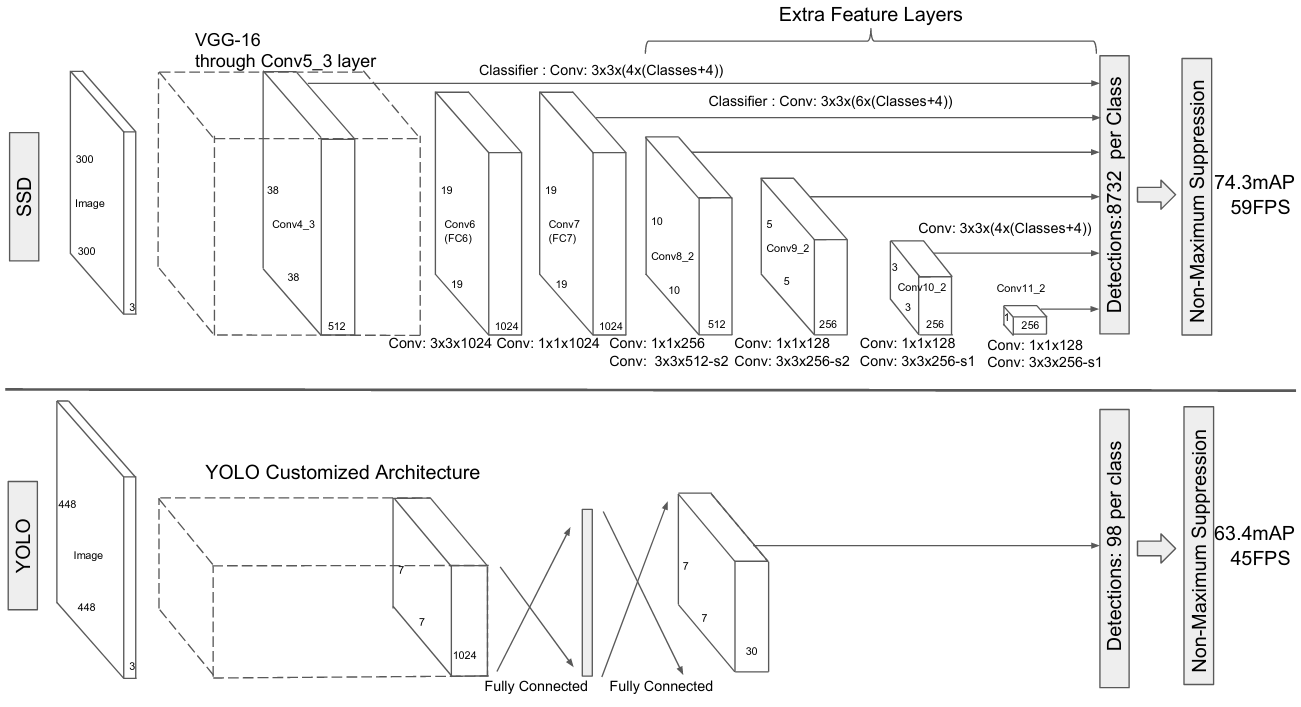
\includegraphics[width=0.8\linewidth]{arch_ssd_yolo}
	\caption{General architecture of a SSD network (top) and a YOLO one (bottom).}
	\label{fig:1_arch_ssd_yolo}
\end{figure}


\subsection{Person identification}
On a controlled environment, where the only present person is the one to be followed, a person detection system could be enough for following purposes. However, in a regular scenario, there might be several people inside the field of vision of the robot. This problem can be approached by means of a distinguishing feature of the person of interest, provided beforehand. One example is \cite{color_id}, which computes the color distribution of the person of interest, and later compares this distribution with the ones belonging to the different persons using the Bhattacharyya coefficient \cite{bhattacharyya} (a measurement of similarity between two probability distributions). This metric can be applied to measuring the similarity between the color histograms of the reference person and the detected one. However, this system can be deceived replicating the color distribution of the person of interest: wearing similar clothes helps to reduce the distance between the histogram, leaving a chance to confound another person with the one to follow.\\

A more robust approach is to use the \textit{face} of the person as the discriminant feature, as its uniqueness makes it a good reference to identify the detected person. As it is summarized in \cite{dlib_review}, several applications extract facial \textit{landmarks} from the morphology of a given face (\autoref{fig:1_dlib_landmarks}), and use them to classify the face, comparing it against a set of known faces and estimating the identity based on the distance to each known face. Some open-source libraries such as \texttt{dlib} and \texttt{OpenCV} provide the algorithms to perform these processes.\\

\begin{figure}[h]
	\centering
	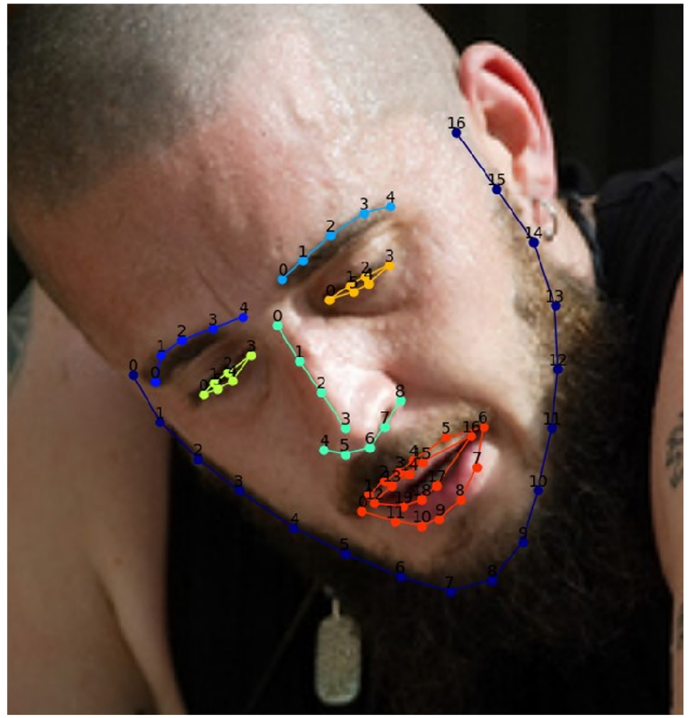
\includegraphics[width=0.6\linewidth]{dlib_landmarks}
	\caption{Facial landmarks are dependent of the face shape and morphology (image from \cite{dlib_review}).}
	\label{fig:1_dlib_landmarks}
\end{figure}


The intuition behind these methods are to \textit{project} the image of the face into a lower dimensionality space, which allows to extract significant features from each face. These features have to be consistent for the same face across different pose and lighting conditions (\autoref{fig:1_faces_poses}). An useful transformation when a dimensionality reduction is pursued is PCA (\textit{Principal Component Analysis}), a linear transformation that can be implemented to deal with the face recognition problem \cite{face_pca}.

\begin{figure}[h]
	\centering
	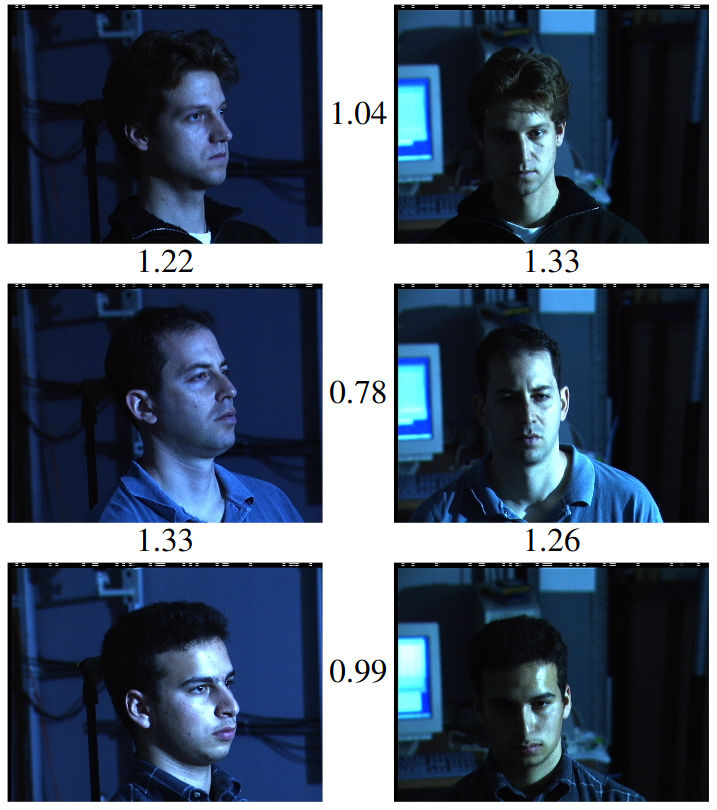
\includegraphics[width=0.40\linewidth]{face_poses}
	\caption{Examples of poses and light conditions across which the face projections are desired to be consistent for the same person (image from \cite{facenet}).}
	\label{fig:1_faces_poses}
\end{figure}
\vspace{4cm}
\subsubsection{Deep learning face identification: FaceNet}
\label{sec:1_facenet}
However, once again neural networks can be leveraged in order to achieve this and more: as the PCA is a linear operation, it could be learned by a single layer neural network. Thus, the introduction of deep networks can yield interesting results. The most relevant approach so far uses deep convolutional networks for performing this process \cite{facenet}, implementing an architecture called \textit{FaceNet}, which is partially based on the Inception \cite{inception} module, designed by Google researchers in order to greatly reduce the number of parameters in a neural network. What this network computes is called an \textit{embedding}, a projection of the input face image into a point in a 128-dimensional hypersphere. This allows to translate the identification into linear algebra terms, such as \textit{distance} between two faces, as well as clustering and applying unsupervised algorithms in order to determine the identity of a trivial face, among a collection of known regions. The architecture can be visualized in \autoref{fig:1_facenet_architecture}. These networks can be trained using a loss function called \textit{triplet loss}, inspired by the work in \cite{lmnn_loss}. Given a training sample (\textit{anchor}), a \textit{positive} example (same class than the anchor) and a \textit{negative} example (different class than the anchor) are chosen, and the network is tuned to maximize the \textit{anchor-negative} embeddings distance, and minimize at the same time the \textit{anchor-positive} one (\autoref{fig:1_facenet_triplet_loss}).


\begin{figure}[h]
	\centering
	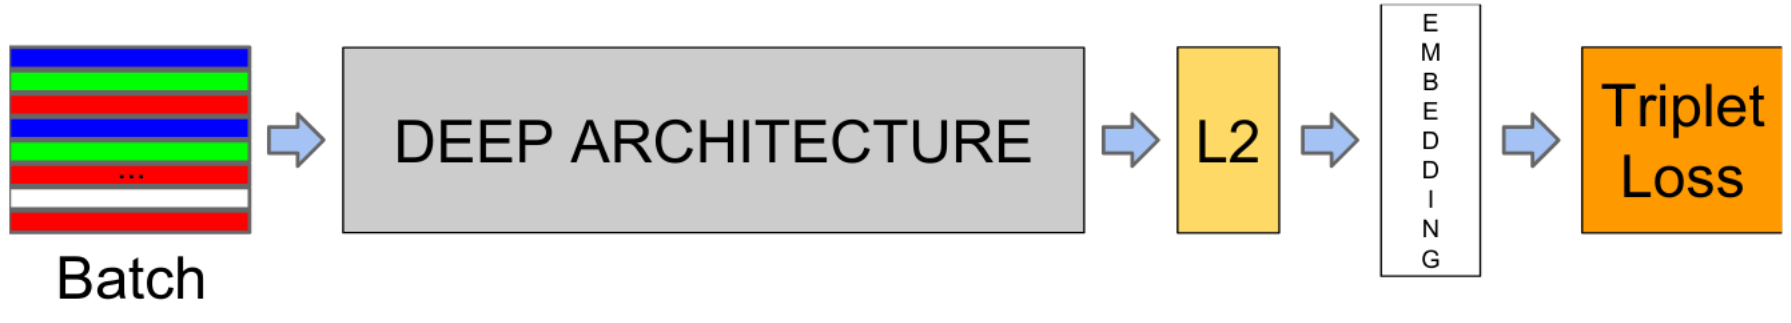
\includegraphics[width=0.7\linewidth]{facenet_architecture}
	\caption{Architecture of the FaceNet system (from \cite{facenet}).}
	\label{fig:1_facenet_architecture}
\end{figure}



\begin{figure}[h]
	\centering
	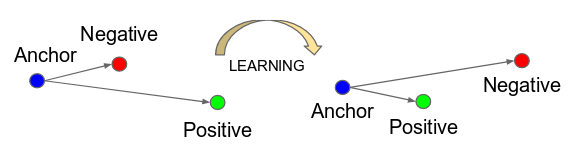
\includegraphics[width=0.7\linewidth]{facenet_triplet_loss}
	\caption{Triplet loss training. It minimizes the distance between an \emph{anchor} (current example) and a \emph{positive}, both of which have the same identity, and maximizes the distance between the \emph{anchor} and a \emph{negative} of a different identity (from \cite{facenet}).}
	\label{fig:1_facenet_triplet_loss}
\end{figure}


One thing to mention about the algorithms described above is that they perform the operations on the image of a face. Thus, a face detection is required for previously cropping the face of the person to be identified. Once again, a neural approach can be reduced to an \textit{object detection} problem (detecting the class \textit{face}, in this case). One interesting approach using this technique is \textit{faced} \cite{faced}. This is a custom small ensemble of two neural networks, responsible to detect faces and correct the bounding boxes found. The main objective of the system is \textit{speed}, so the main detector architecture is based in YOLO \cite{yolov1}, and the second correction stage raises the precision achieved by the detector, achieving better results than a classical Haar approach, as it can be seen on \autoref{fig:1_faced_vs_haar}. Further comparisons are performed on \autoref{chap:3_results} between these two detection methods.

\begin{figure}[h]
	\centering
	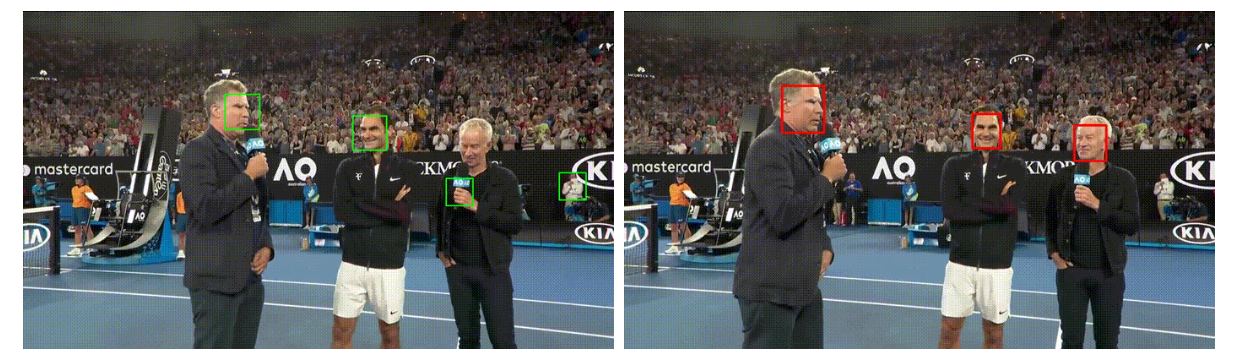
\includegraphics[width=0.8\linewidth]{faced_vs_haar}
	\caption{Classical Haar based face detector \cite{violajones} (left) vs. \textit{faced} (right). Image from \cite{faced}.}
	\label{fig:1_faced_vs_haar}
\end{figure}


\subsection{Embedded deployment}
One of the requirements of this work is to be integrated in an autonomous robot. This imposes a power limitation on the algorithms to be deployed. Generally, the robotic systems are deployed using laptops connected to robots, as it was done in \cite{tfg}.

\begin{figure}[h]
	\centering
	\begin{subfigure}[h]{0.4\linewidth}
		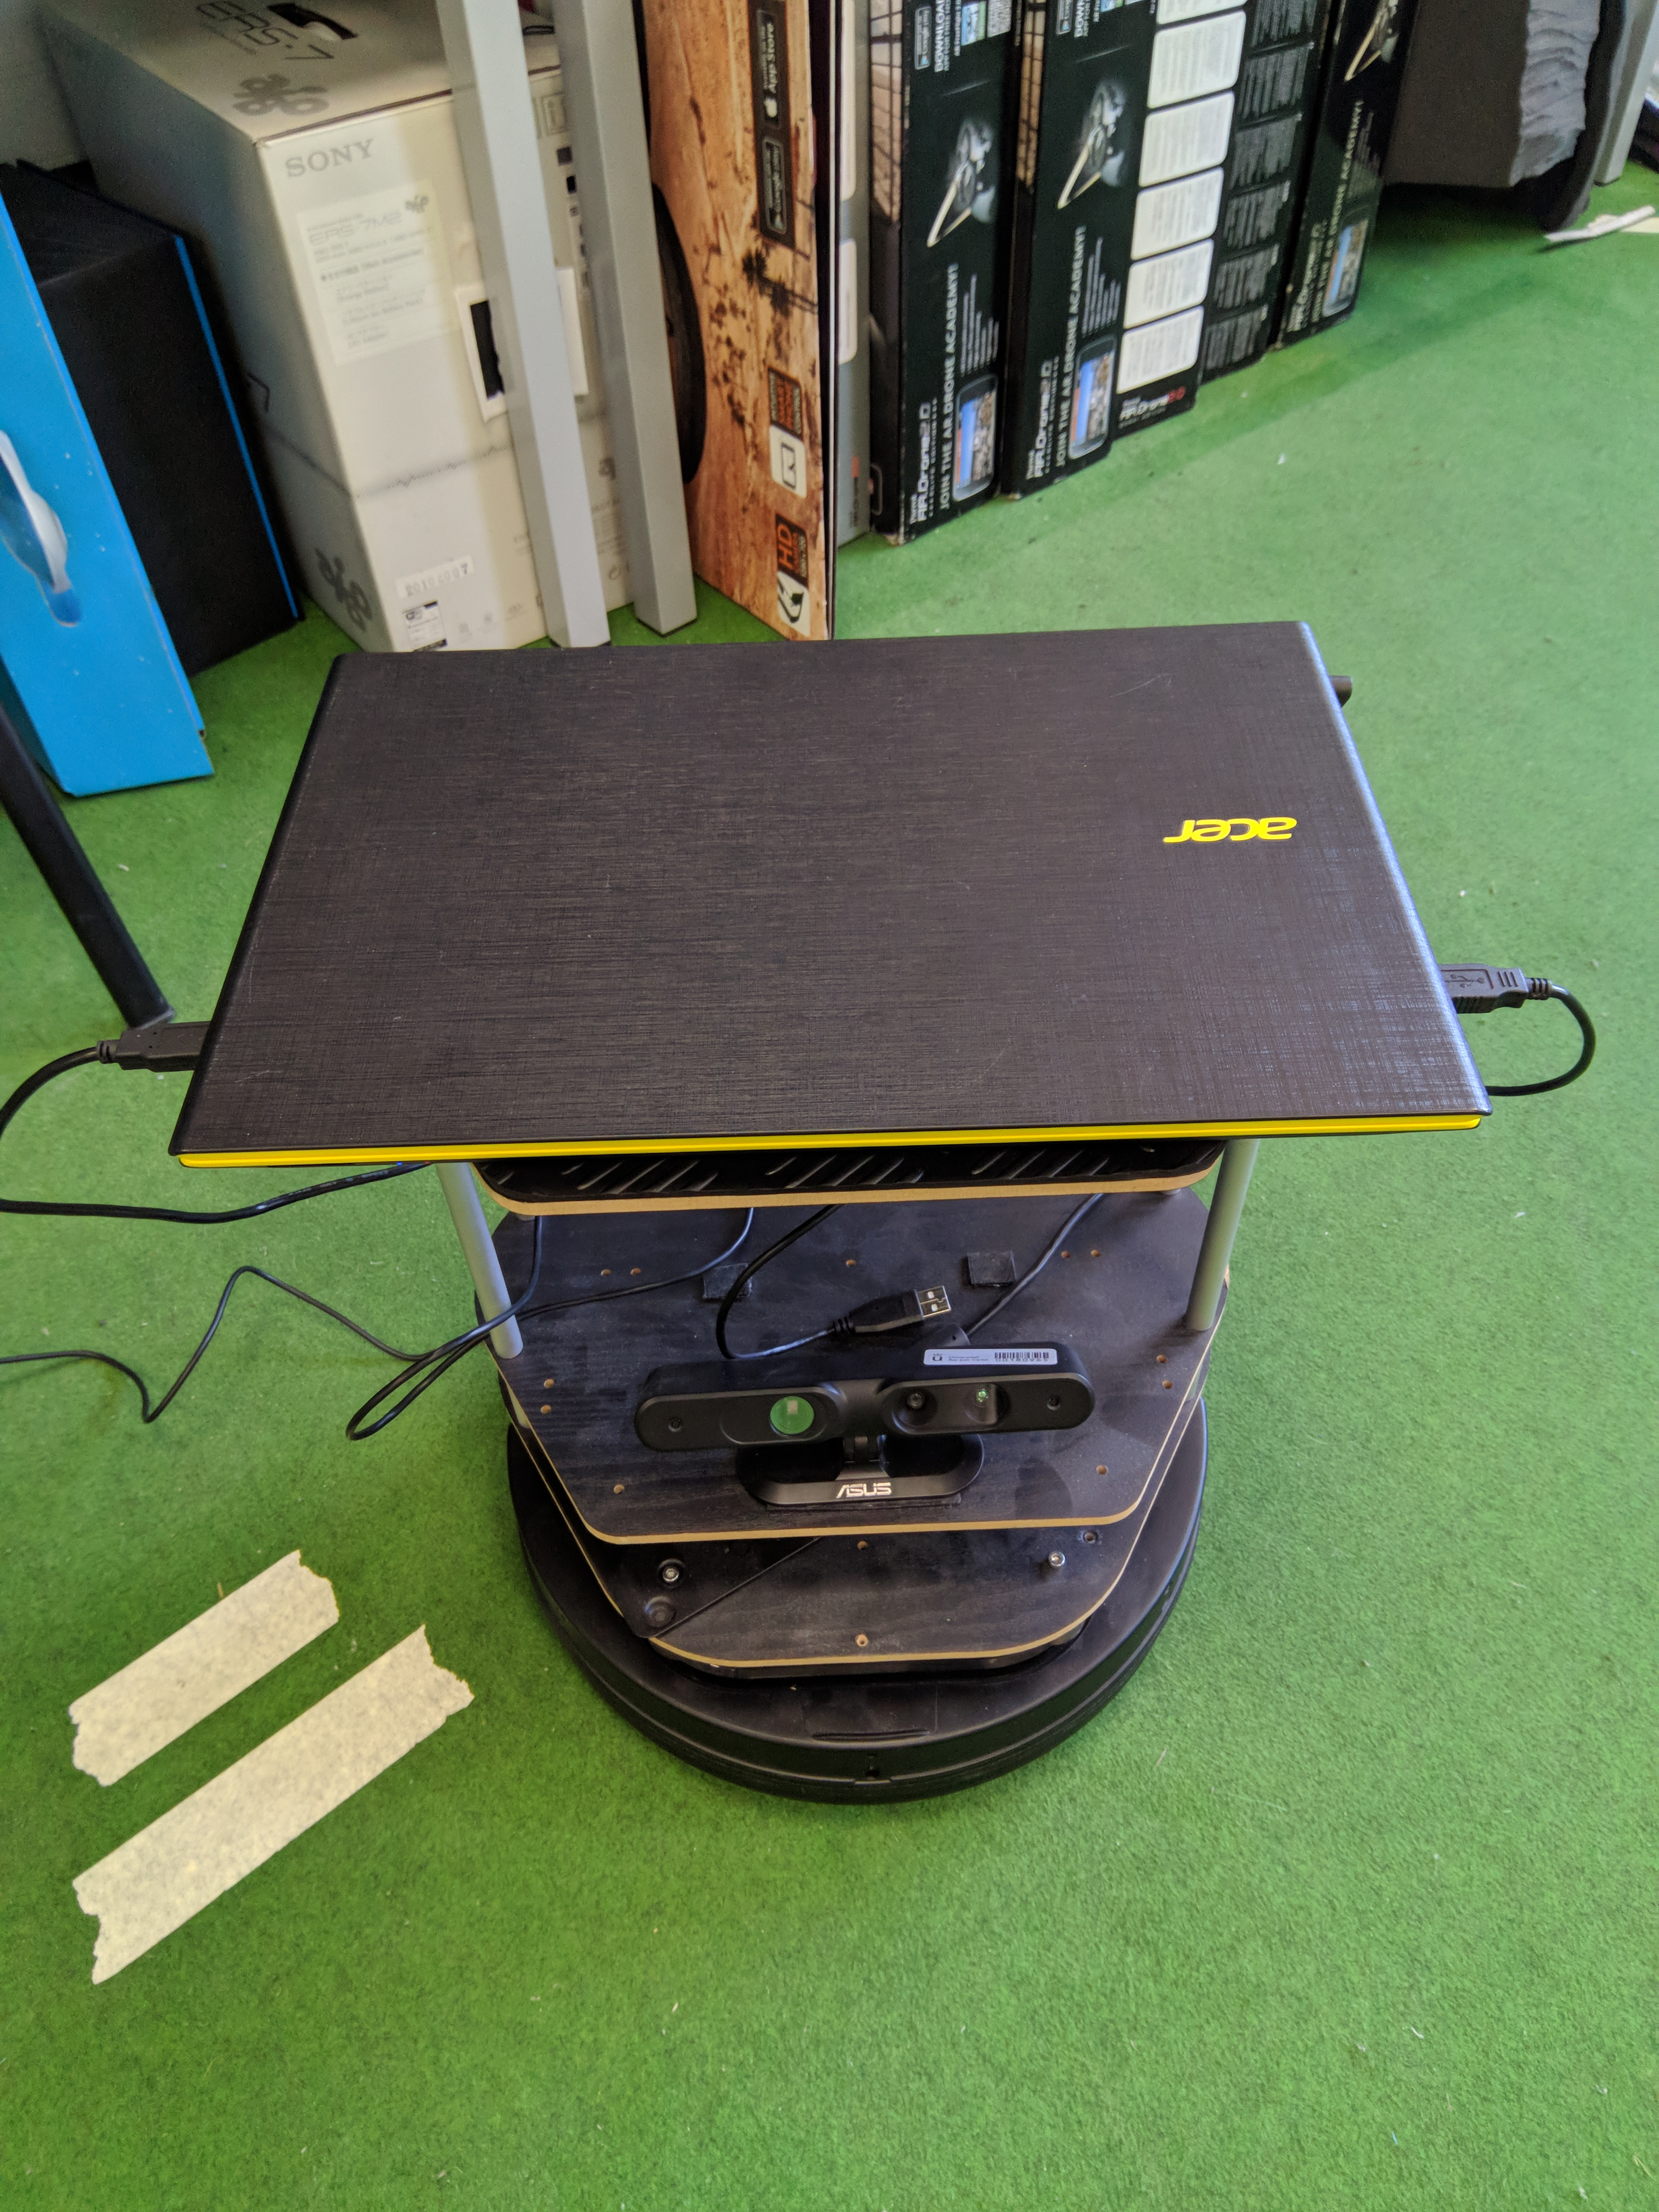
\includegraphics[width=1.9in]{tfg1}
		\caption{Frontal view.}
		\label{fig:1_turtlebot_front}
	\end{subfigure}
	\begin{subfigure}[h]{0.4\linewidth}
		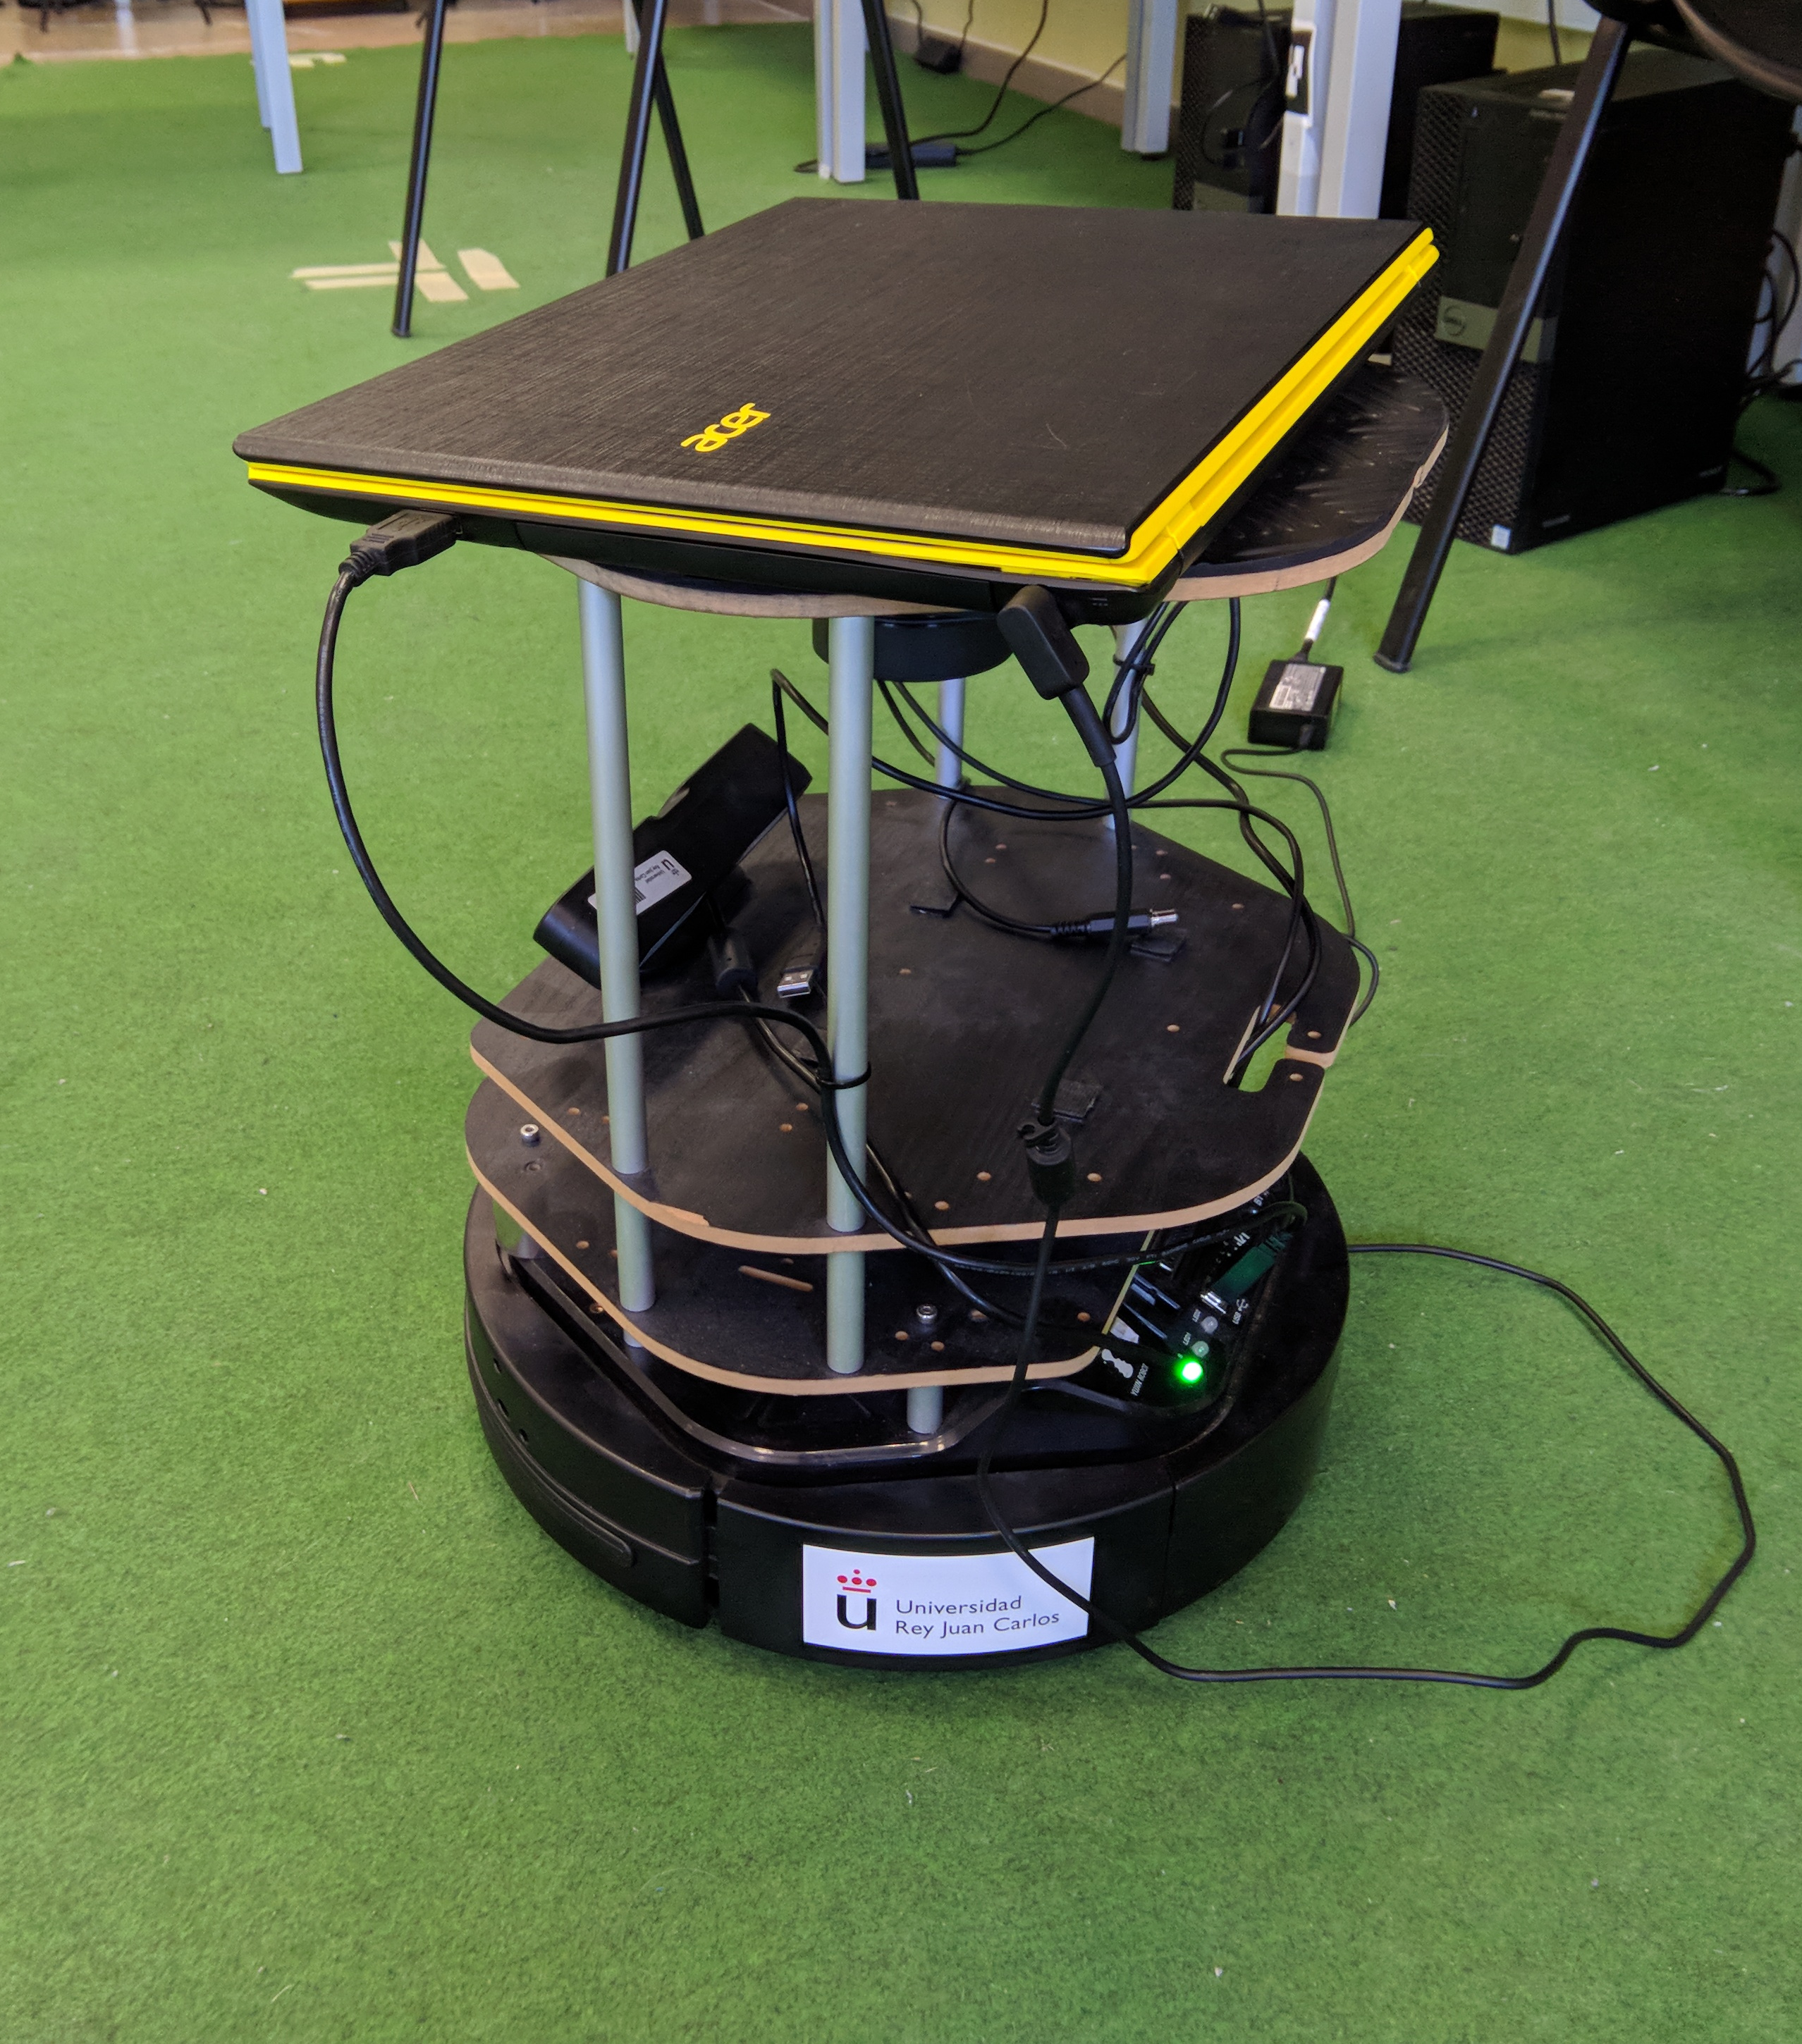
\includegraphics[width=2.2in]{tfg2}
		\caption{Side view.}
		\label{fig:1_turtlebot_side}
	\end{subfigure}
	\caption{Laptop+robot deployment on \cite{tfg}.}
	\label{fig:1_real_tfg}
\end{figure}

Nowadays, the mentioned increase in the interest into the real-time computer vision applications has fostered the development of specific low-power embedded devices to be integrated in mobile systems. The extending usage of devices such as Arduino or Raspberry Pi has led to embedded robotics systems, such as PiBot \cite{pibot} (\autoref{fig:1_pibot}). These robots are useful in the educational scope, as they are capable of running simple vision and navigation algorithms at a low cost.\\
\begin{figure}[h]
	\centering
	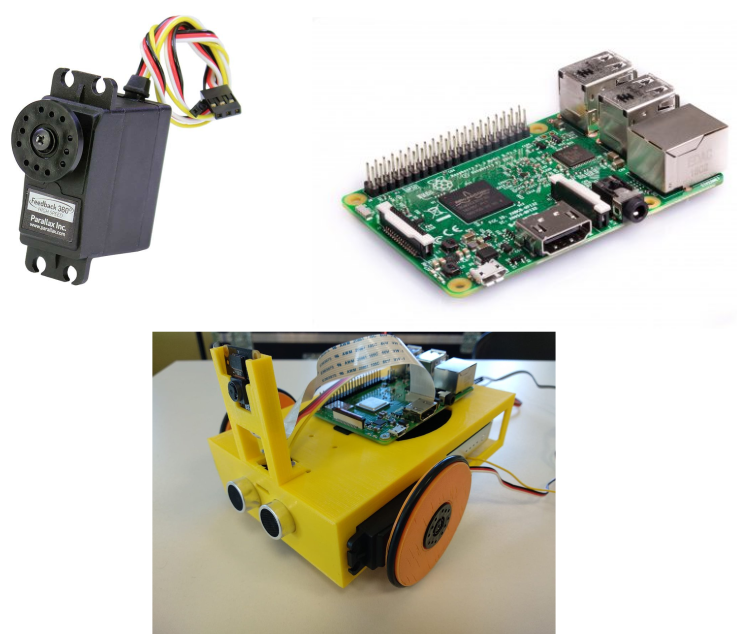
\includegraphics[width=0.5\linewidth]{pibot}
	\caption{PiBot, an open low-cost robotic platform for education (image from \cite{pibot}).}
	\label{fig:1_pibot}
\end{figure}
Unfortunately, the requirements for running more complex algorithms, such as neural networks, require of the next tier in power terms, keeping the portability nevertheless. The ideal device could be an ASIC, as the custom design would lead to a very tight optimization of the performance. However, the objective is to run the algorithms on existing software frameworks, requiring to use general purpose computers instead. The most remarkable advance in this scope are the Jetson devices manufactured by NVIDIA. These development boards are SoM computers running a tailored version of Linux. The fundamental feature of these systems is that they include a high-performance GPU featuring CUDA, a low-level parallel computation library, as well as several toolkits (such as TensorRT\footnote{\url{https://developer.nvidia.com/tensorrt}}) designed to optimize as much as possible the software implementations for the plethora of possibilities to be designed on this board. As it can be seen in \autoref{fig:1_tx2}, its size and power consumption make this system a good choice to be included in an autonomous robot. 
\begin{figure}[h!]
	\begin{subfigure}[h]{0.45\linewidth}
		\centering
		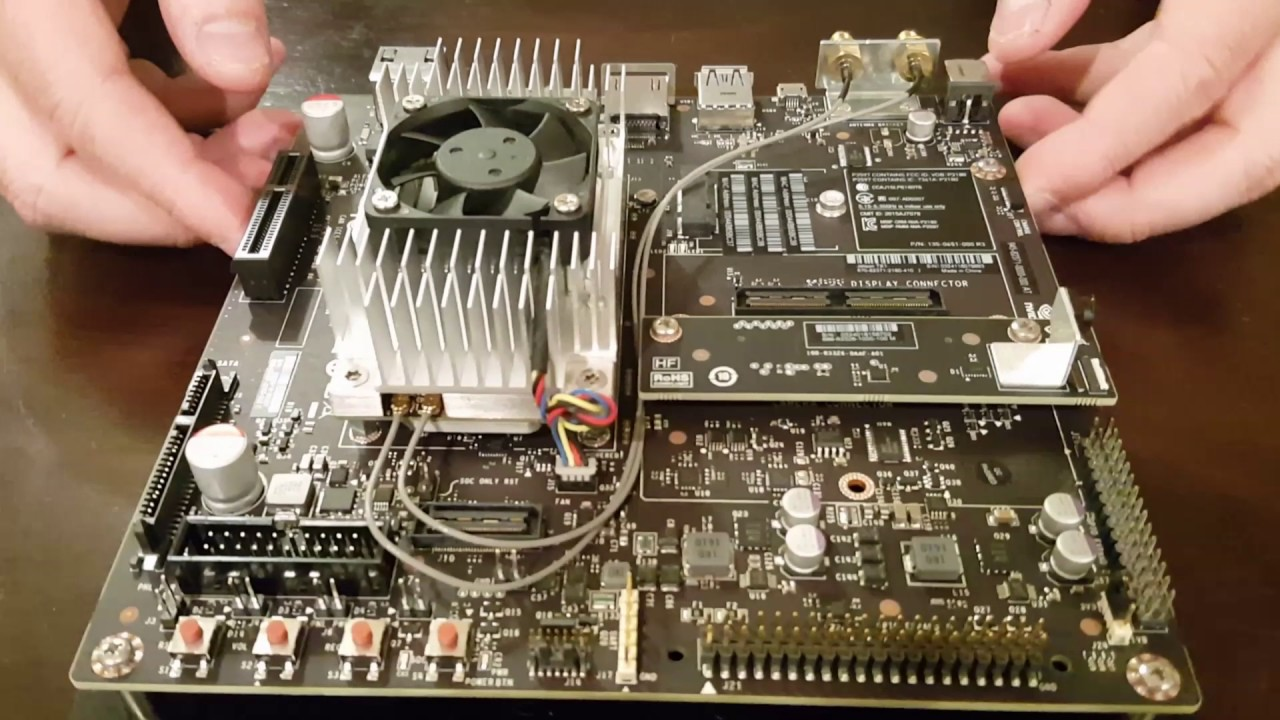
\includegraphics[width=\linewidth]{jetsontx2}

	\end{subfigure}
	\begin{subfigure}[h]{0.45\linewidth}
		\centering
		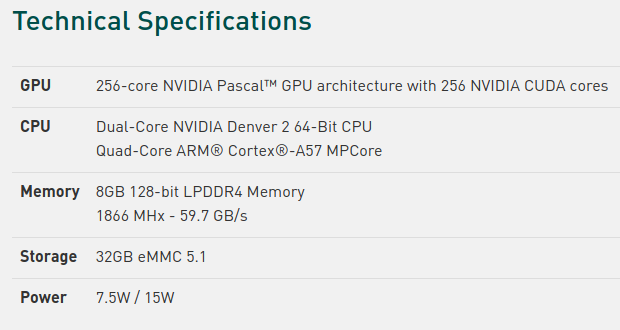
\includegraphics[width=\linewidth]{tx2_specs}
	\end{subfigure}
	\caption{NVIDIA Jetson TX2: an embedded high-performance device including a GPU.}
	\label{fig:1_tx2}
\end{figure}


\subsection{Person following}
Several approaches have been developed pursuing this challenge of \textit{following a person}. Once the perception algorithms are established, the final output of the pipeline has to be a movement command for the robot to move towards the desired point. Mobile  robots can be classified according to their locomotion capabilities. A robot is \textit{holonomic} if the number of its controllable degrees of freedom is equal to its total degrees of freedom. If the controllable degrees of freedom are lower than the total degrees of freedom, the robot is \textit{non-holonomic}. This difference can be observed on \autoref{fig:1_holonomics}. In the case of a holonomic robot, the navigation process is simplified, as the robot can instantaneously move to a desired target. However, a non-holonomic robot needs to perform maneuvers in order to move towards a point.\\


\begin{figure}[h]
	\centering
	\begin{subfigure}[t]{0.45\linewidth}
		\centering
		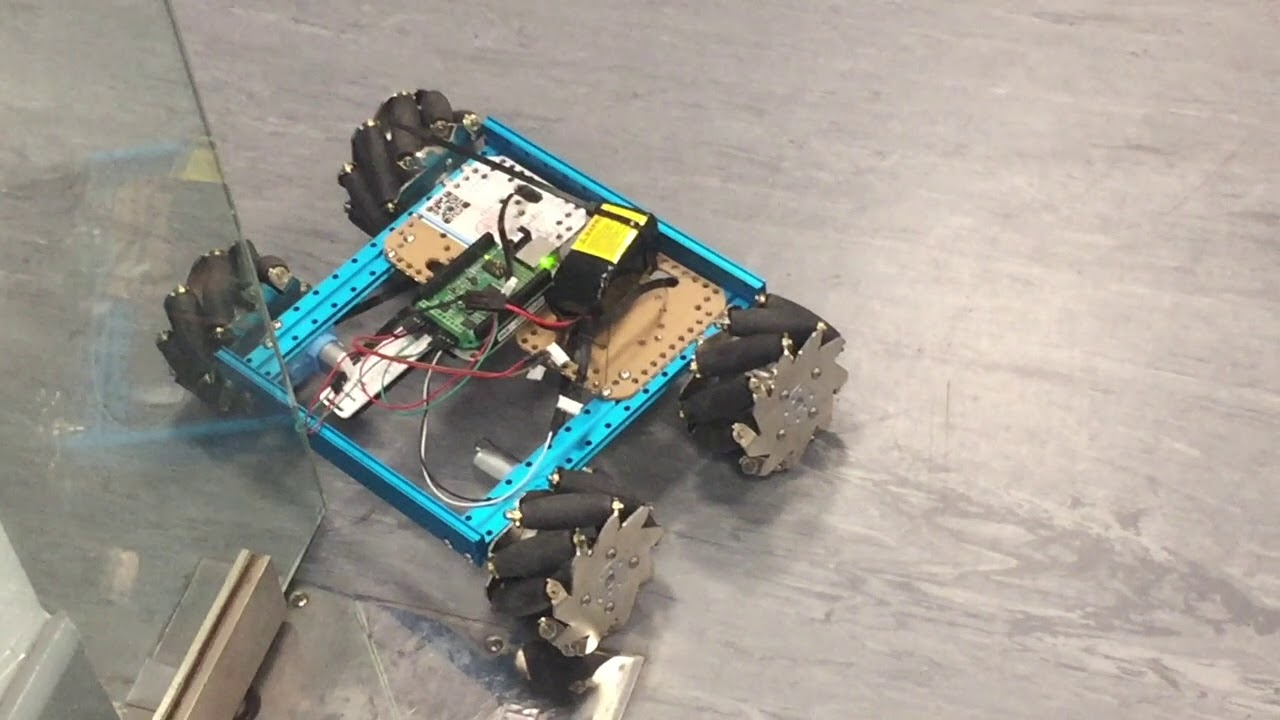
\includegraphics[width=\linewidth]{holonomic_robot}
		\caption{Holonomic robot.}
	\end{subfigure}
	\begin{subfigure}[t]{0.45\linewidth}
	\centering
	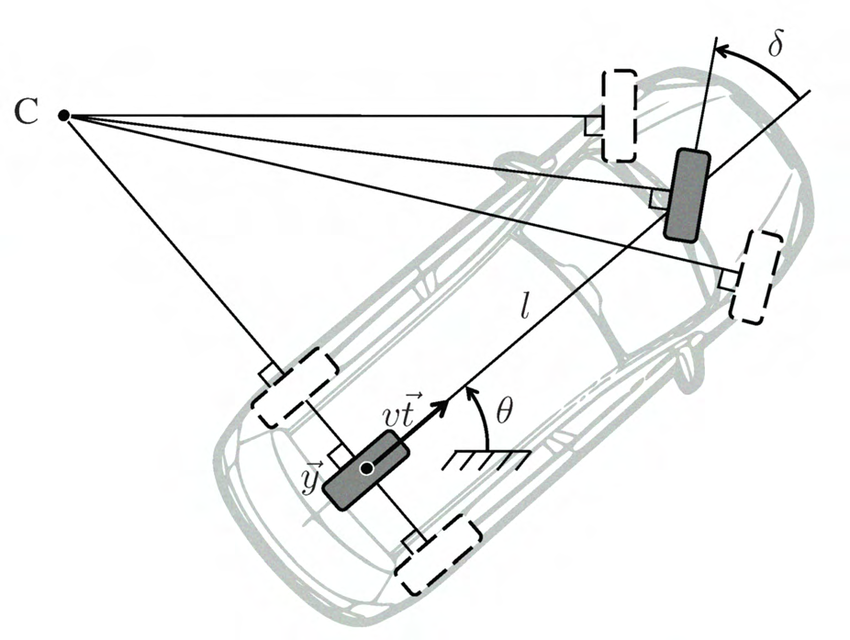
\includegraphics[width=\linewidth]{non_holonomic_robot}
	\caption{Schematic of the degrees of freedom of a non-holonomic vehicle (a standard car).}
	\end{subfigure}
	\caption{Comparison of a holonomic system with a non-holonomic one.}
	\label{fig:1_holonomics}
\end{figure}

The summary on \cite{personfollowing_summary} shows an interesting classification of some existing person following algorithms and their applications (\autoref{fig:1_personfollowing_summary}).


\begin{figure}[h]
	\centering
	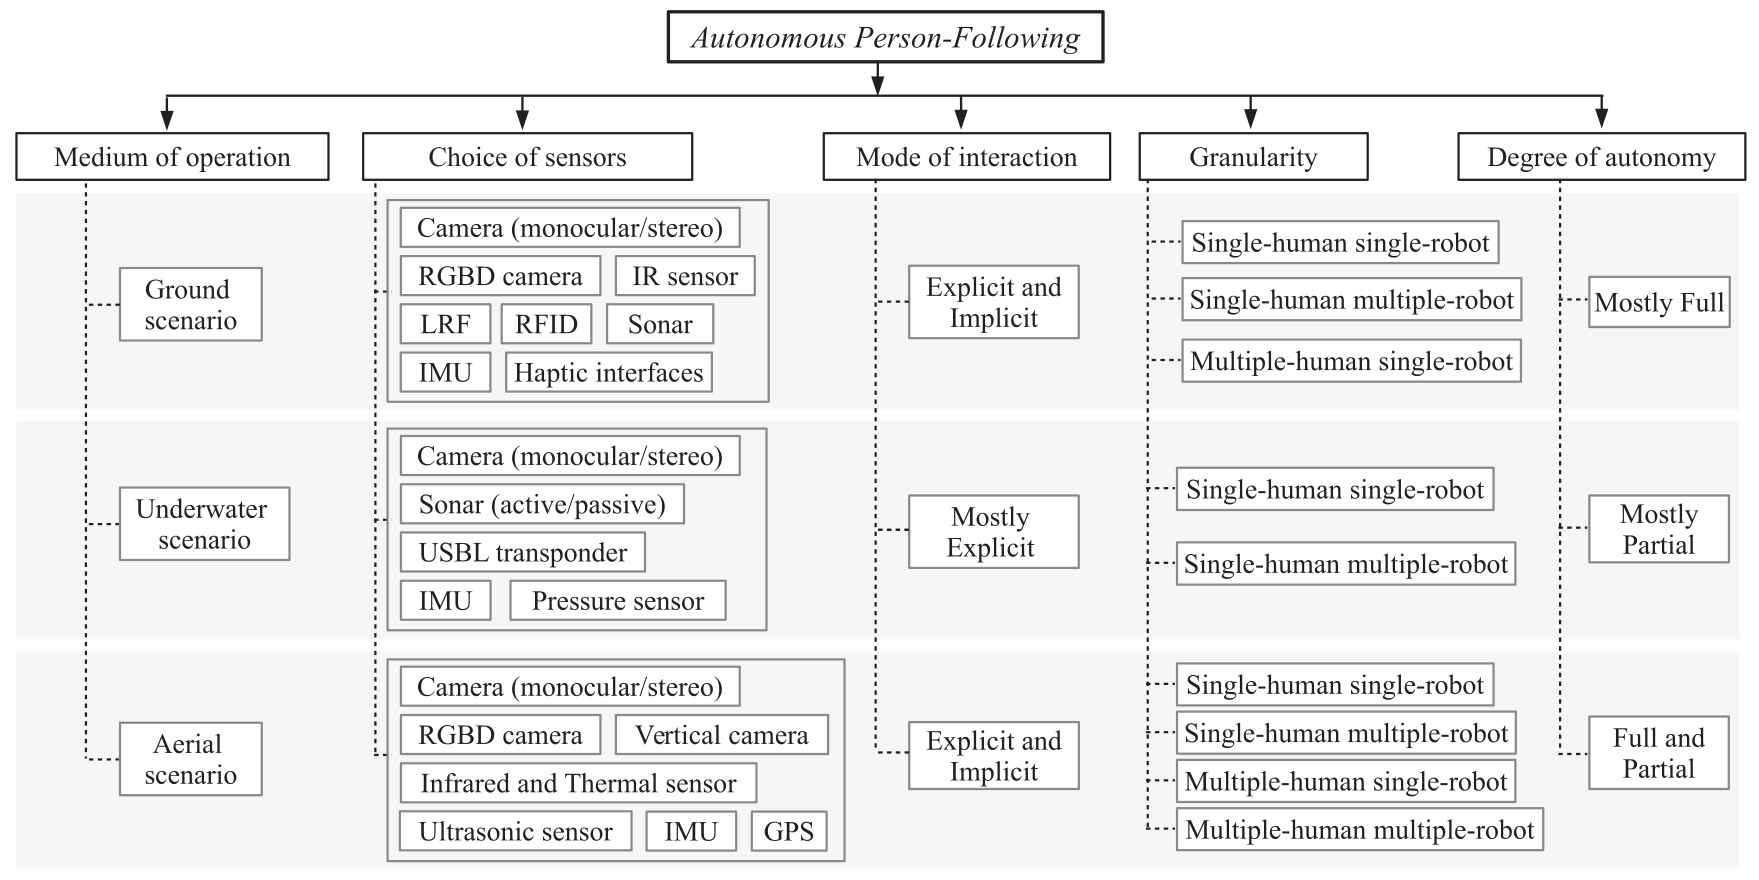
\includegraphics[width=\linewidth]{personfollowing_summary}
	\caption{In-depth classification of the existing person following algorithms (image from \cite{personfollowing_summary}).}
	\label{fig:1_personfollowing_summary}
\end{figure}

Some approaches leverage the detected objects in order to estimate the relative homography of the orthogonal planes, which allows to partially know the environment of the robot and trace a safe path towards the person, as it can be seen on \autoref{fig:1_personfollowing_homography}.

\begin{figure}
	\centering
	\begin{subfigure}[t]{0.45\linewidth}
		\centering
		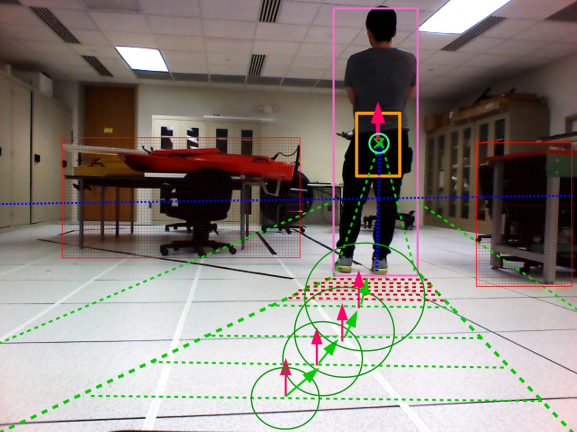
\includegraphics[width=0.95\linewidth]{personfollowing_homography}
		\caption{Following with path computation using homographies (image from \cite{personfollowing_summary}).}
		\label{fig:1_personfollowing_homography}
	\end{subfigure}
	\begin{subfigure}[t]{0.45\linewidth}
		\centering
		
		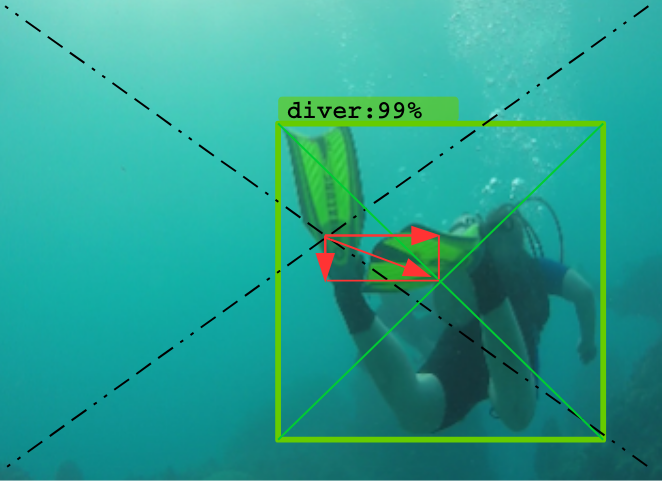
\includegraphics[width=0.95\linewidth]{personfollowing_reactive}
		\caption{Example of underwater reactive following (image from \cite{personfollowing_reactive}).}
		\label{fig:1_personfollowing_reactive}
	\end{subfigure}
\end{figure}



Other approaches act without a path planning component, implementing what is called a \textit{reactive} behavior \cite{personfollowing_reactive}, similar to the proposed solution  on this work. On these approaches, the vector between the center of the image and the center of the person is used to command movements on the robot, as it can be seen on \autoref{fig:1_personfollowing_reactive}.

\newpage
\section{Objectives}
\label{sec:1_objectives}

	The main objective of this work is to design and develop an embedded system which allows a low-cost robot with a camera to follow a certain person on a robust way. The result will be an autonomous robot which will follow a specific person, whose face has to be known beforehand (using a \textit{reference face} image). This objective, in turn, can be split into specific subgoals:
	
	\begin{enumerate}
		\item Implement a real-time person following behavior using embedded low-power hardware and a low-complexity educational robot.
		
		\item Build the inference pipeline using exclusively concurrent CNNs (\textit{convolutional neural networks}), as they offer robustness on detection under harsh lighting conditions, such as the ones observed in \autoref{fig:1_light_ko}.
		
		\begin{figure}[h]
			\centering
			\begin{subfigure}[b]{0.3\linewidth}
				\centering
				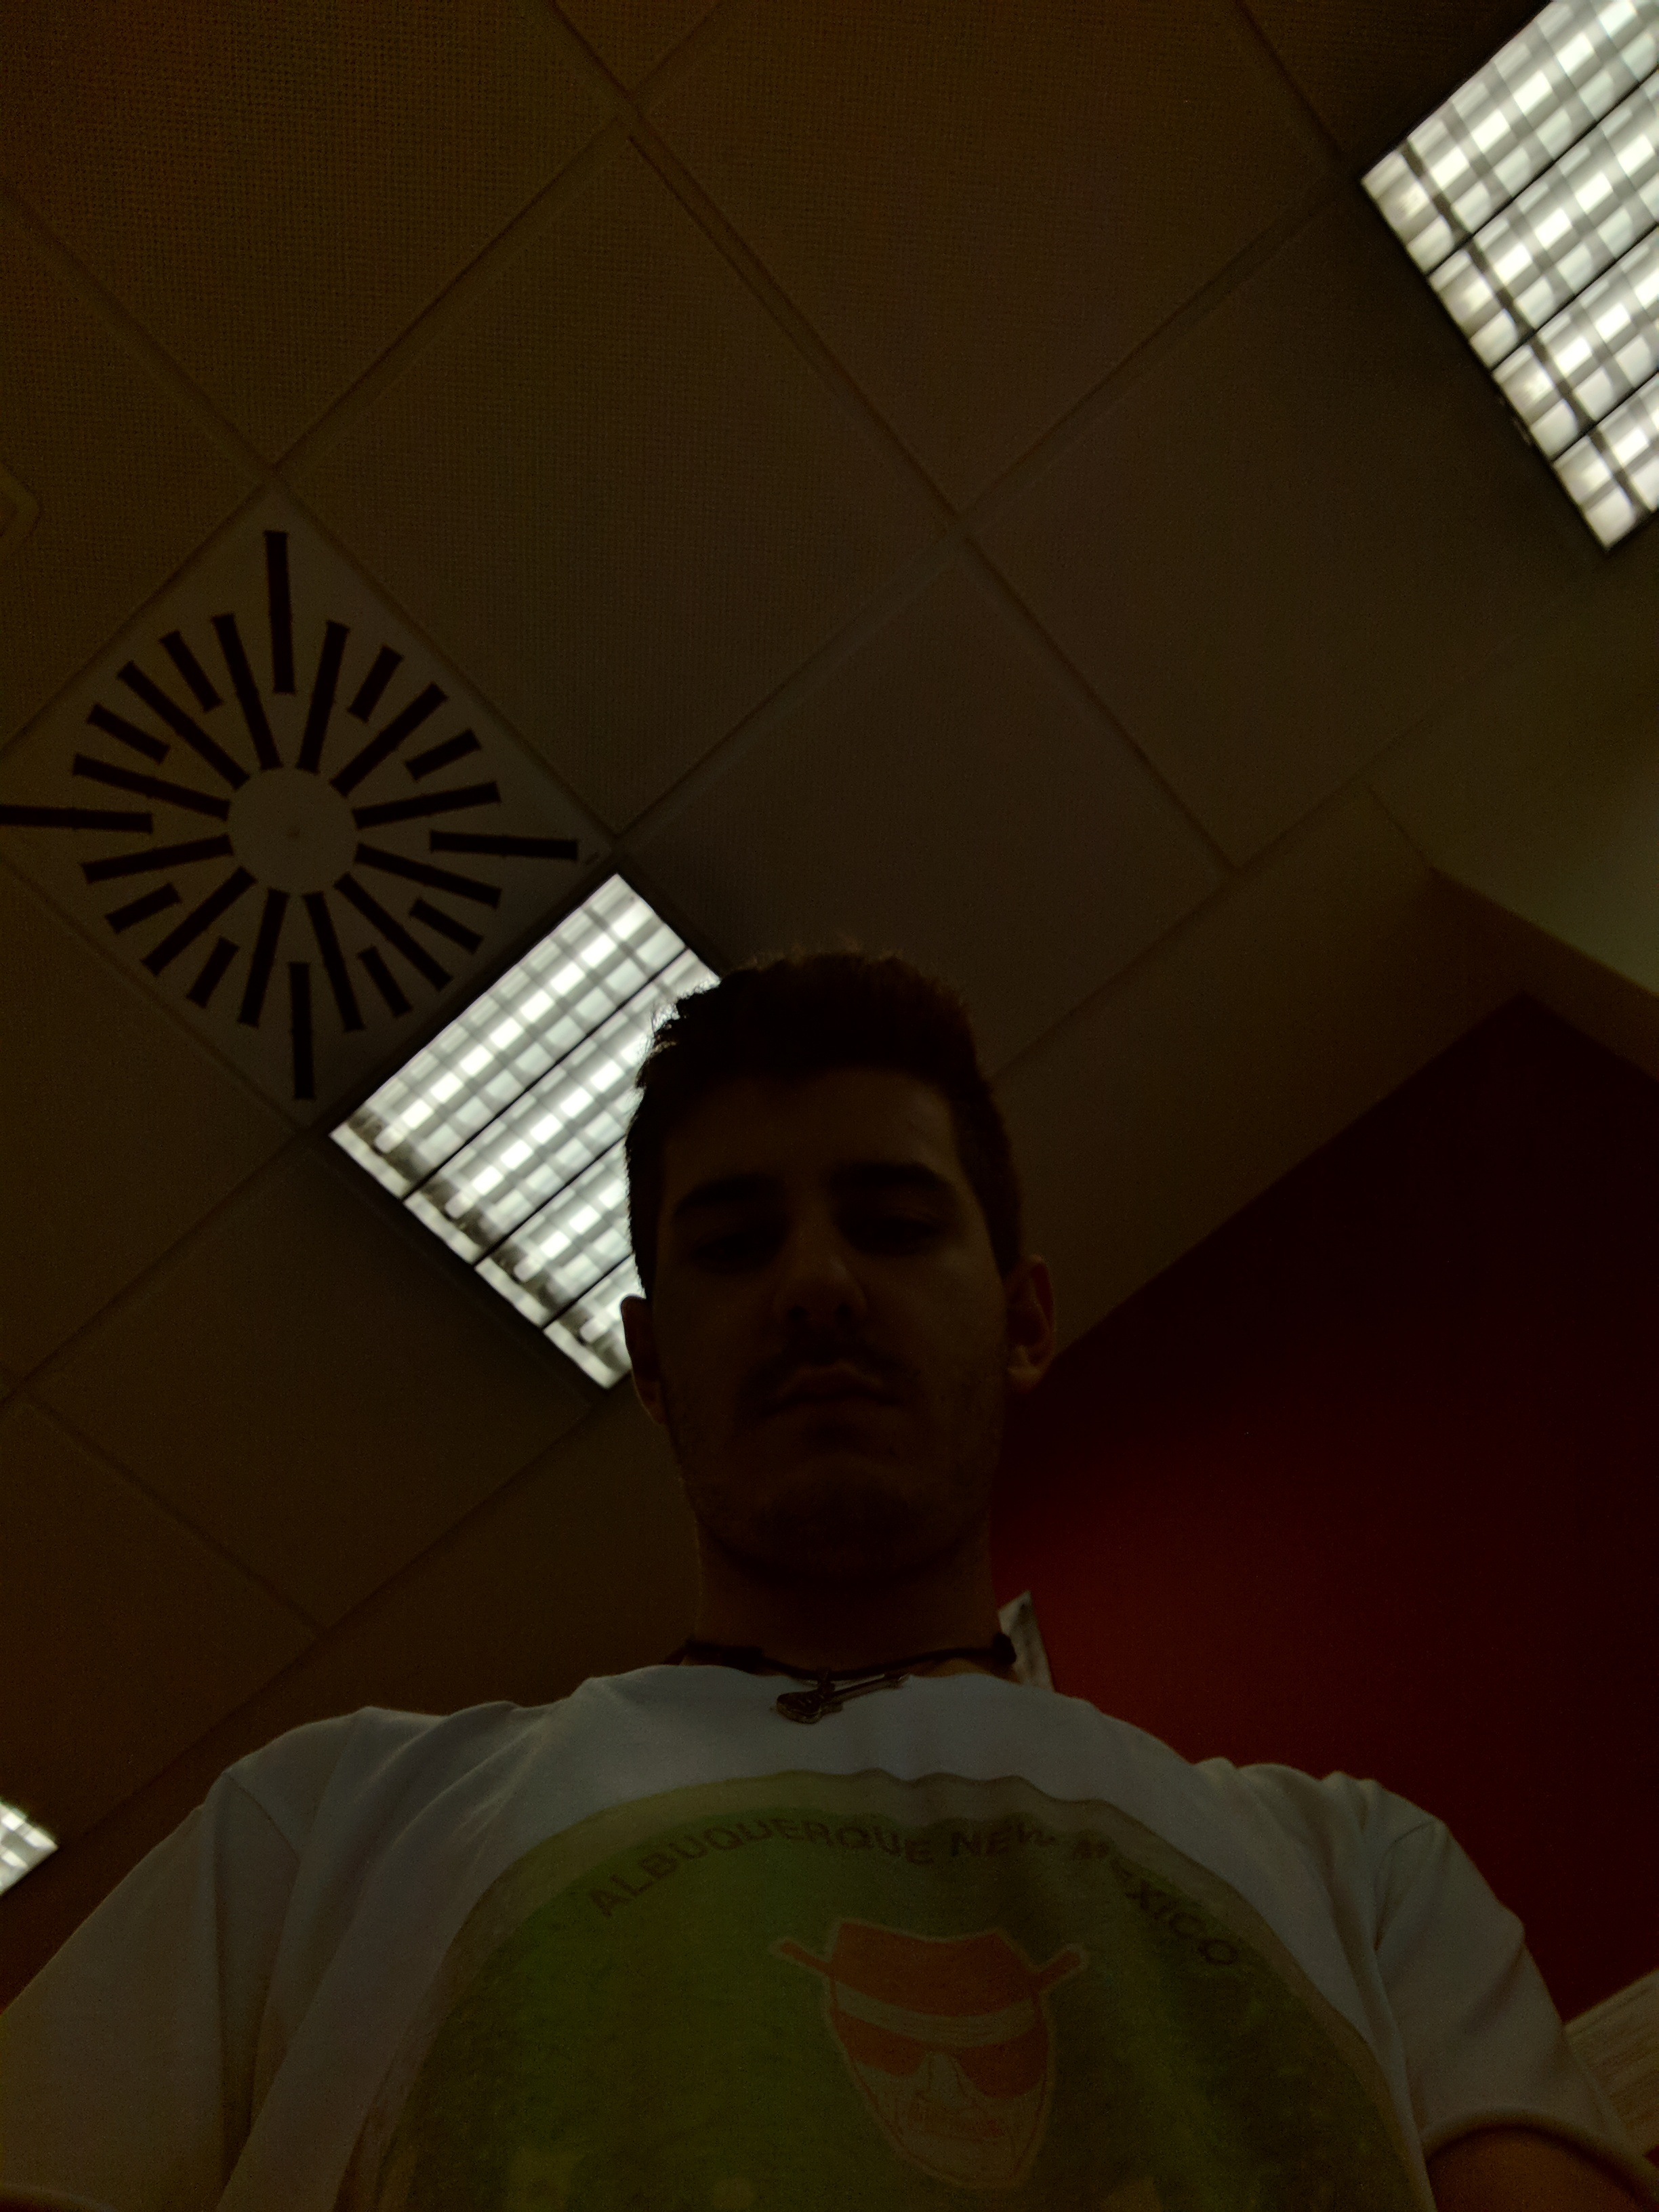
\includegraphics[width=\linewidth]{light_ko}
			\end{subfigure}
			\hfill
			\begin{subfigure}[b]{0.5\linewidth}
				\centering
				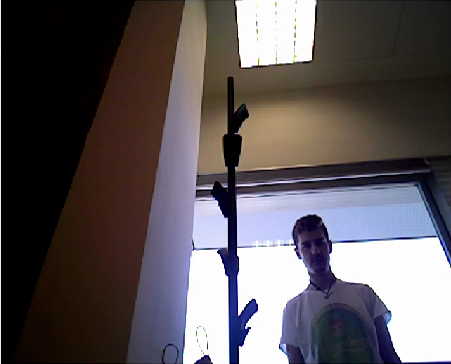
\includegraphics[width=\linewidth]{light_ko_2}
			\end{subfigure}		
			
			\caption{Poor lighting situations for a low-positioned camera.}
			\label{fig:1_light_ko}
		\end{figure}
		
		
		\item Combine a neural visual perception with optical tracking to carry out a robust following of the persons in front of the robot. This will provide the system with extra reliability and robustness against detection losses/occlusions.
	\end{enumerate}
	
These subgoals allow to summarize the starting point for the development of this project: the available materials are an educational robot equipped with a battery, an embedded \textit{SoM} and a RGB-D sensor.\\


The structure of this work is organized as follows:
\begin{itemize}
	\item Chapter \ref{chap:1_introduction} presents the motivation of this work, as well as the framework into which it can be placed. Finally, the objectives to be addressed are specified.
	\item Chapter \ref{chap:2_materials_methods} describes the hardware and software means of the developed work. Later, a full functional description of the implemented system is depicted, describing the \textit{Perception} and \textit{Actuation} modules that compose the system. Finally, a description is performed on the software architecture that implements the following behavior and makes the robot to follow the person.
	\item Chapter \ref{chap:3_results} describes the experiments conducted on the subsystems and modules of this work. The results of each test are shown as well in order to demonstrate the convenience of the design decisions taken along the development. Finally, a global system experiment is shown, where the robot can be seen on its following behavior.
	\item Chapter \ref{chap:4_discussions} discusses the obtained results on the experiments. Later, conclusions are drawn from the developed work, revisiting the goals and subgoals presented above, and proposing future lines of work that can improve the robot and address its main drawbacks.
\end{itemize}


